\documentclass[twoside]{book}

% Packages required by doxygen
\usepackage{fixltx2e}
\usepackage{calc}
\usepackage{doxygen}
\usepackage[export]{adjustbox} % also loads graphicx
\usepackage{graphicx}
\usepackage[utf8]{inputenc}
\usepackage{makeidx}
\usepackage{multicol}
\usepackage{multirow}
\PassOptionsToPackage{warn}{textcomp}
\usepackage{textcomp}
\usepackage[nointegrals]{wasysym}
\usepackage[table]{xcolor}

% Font selection
\usepackage[T1]{fontenc}
\usepackage[scaled=.90]{helvet}
\usepackage{courier}
\usepackage{amssymb}
\usepackage{sectsty}
\renewcommand{\familydefault}{\sfdefault}
\allsectionsfont{%
  \fontseries{bc}\selectfont%
  \color{darkgray}%
}
\renewcommand{\DoxyLabelFont}{%
  \fontseries{bc}\selectfont%
  \color{darkgray}%
}
\newcommand{\+}{\discretionary{\mbox{\scriptsize$\hookleftarrow$}}{}{}}

% Page & text layout
\usepackage{geometry}
\geometry{%
  a4paper,%
  top=2.5cm,%
  bottom=2.5cm,%
  left=2.5cm,%
  right=2.5cm%
}
\tolerance=750
\hfuzz=15pt
\hbadness=750
\setlength{\emergencystretch}{15pt}
\setlength{\parindent}{0cm}
\setlength{\parskip}{0.2cm}
\makeatletter
\renewcommand{\paragraph}{%
  \@startsection{paragraph}{4}{0ex}{-1.0ex}{1.0ex}{%
    \normalfont\normalsize\bfseries\SS@parafont%
  }%
}
\renewcommand{\subparagraph}{%
  \@startsection{subparagraph}{5}{0ex}{-1.0ex}{1.0ex}{%
    \normalfont\normalsize\bfseries\SS@subparafont%
  }%
}
\makeatother

% Headers & footers
\usepackage{fancyhdr}
\pagestyle{fancyplain}
\fancyhead[LE]{\fancyplain{}{\bfseries\thepage}}
\fancyhead[CE]{\fancyplain{}{}}
\fancyhead[RE]{\fancyplain{}{\bfseries\leftmark}}
\fancyhead[LO]{\fancyplain{}{\bfseries\rightmark}}
\fancyhead[CO]{\fancyplain{}{}}
\fancyhead[RO]{\fancyplain{}{\bfseries\thepage}}
\fancyfoot[LE]{\fancyplain{}{}}
\fancyfoot[CE]{\fancyplain{}{}}
\fancyfoot[RE]{\fancyplain{}{\bfseries\scriptsize Generated on Sun Jun 14 2015 05\+:05\+:19 for My Project by Doxygen }}
\fancyfoot[LO]{\fancyplain{}{\bfseries\scriptsize Generated on Sun Jun 14 2015 05\+:05\+:19 for My Project by Doxygen }}
\fancyfoot[CO]{\fancyplain{}{}}
\fancyfoot[RO]{\fancyplain{}{}}
\renewcommand{\footrulewidth}{0.4pt}
\renewcommand{\chaptermark}[1]{%
  \markboth{#1}{}%
}
\renewcommand{\sectionmark}[1]{%
  \markright{\thesection\ #1}%
}

% Indices & bibliography
\usepackage{natbib}
\usepackage[titles]{tocloft}
\setcounter{tocdepth}{3}
\setcounter{secnumdepth}{5}
\makeindex

% Hyperlinks (required, but should be loaded last)
\usepackage{ifpdf}
\ifpdf
  \usepackage[pdftex,pagebackref=true]{hyperref}
\else
  \usepackage[ps2pdf,pagebackref=true]{hyperref}
\fi
\hypersetup{%
  colorlinks=true,%
  linkcolor=blue,%
  citecolor=blue,%
  unicode%
}

% Custom commands
\newcommand{\clearemptydoublepage}{%
  \newpage{\pagestyle{empty}\cleardoublepage}%
}


%===== C O N T E N T S =====

\begin{document}

% Titlepage & ToC
\hypersetup{pageanchor=false,
             bookmarks=true,
             bookmarksnumbered=true,
             pdfencoding=unicode
            }
\pagenumbering{roman}
\begin{titlepage}
\vspace*{7cm}
\begin{center}%
{\Large My Project }\\
\vspace*{1cm}
{\large Generated by Doxygen 1.8.9.1}\\
\vspace*{0.5cm}
{\small Sun Jun 14 2015 05:05:19}\\
\end{center}
\end{titlepage}
\clearemptydoublepage
\tableofcontents
\clearemptydoublepage
\pagenumbering{arabic}
\hypersetup{pageanchor=true}

%--- Begin generated contents ---
\chapter{Namespace Index}
\section{Namespace List}
Here is a list of all documented namespaces with brief descriptions\+:\begin{DoxyCompactList}
\item\contentsline{section}{\hyperlink{namespacepel}{pel} }{\pageref{namespacepel}}{}
\item\contentsline{section}{\hyperlink{namespaceUi}{Ui} }{\pageref{namespaceUi}}{}
\end{DoxyCompactList}

\chapter{Hierarchical Index}
\section{Class Hierarchy}
This inheritance list is sorted roughly, but not completely, alphabetically\+:\begin{DoxyCompactList}
\item \contentsline{section}{entrada\+Historial}{\pageref{classentradaHistorial}}{}
\item \contentsline{section}{Fecha}{\pageref{classFecha}}{}
\item \contentsline{section}{Nego}{\pageref{classNego}}{}
\item \contentsline{section}{Oficina}{\pageref{classOficina}}{}
\item \contentsline{section}{Owner}{\pageref{classOwner}}{}
\item \contentsline{section}{Peticion}{\pageref{classPeticion}}{}
\item Q\+Dialog\begin{DoxyCompactList}
\item \contentsline{section}{dialog\+Informe}{\pageref{classdialogInforme}}{}
\item \contentsline{section}{dialog\+Login}{\pageref{classdialogLogin}}{}
\item \contentsline{section}{dialog\+Nego}{\pageref{classdialogNego}}{}
\item \contentsline{section}{dialog\+Oficinas}{\pageref{classdialogOficinas}}{}
\item \contentsline{section}{dialog\+Owner}{\pageref{classdialogOwner}}{}
\item \contentsline{section}{dialog\+Peticiones}{\pageref{classdialogPeticiones}}{}
\end{DoxyCompactList}
\item Q\+Main\+Window\begin{DoxyCompactList}
\item \contentsline{section}{main\+Window}{\pageref{classmainWindow}}{}
\end{DoxyCompactList}
\item \contentsline{section}{rank}{\pageref{structrank}}{}
\item \contentsline{section}{pel\+:\+:Vector$<$ T $>$}{\pageref{classpel_1_1Vector}}{}
\item \contentsline{section}{pel\+:\+:Vector$<$ entrada\+Historial $>$}{\pageref{classpel_1_1Vector}}{}
\item \contentsline{section}{pel\+:\+:Vector$<$ Oficina $>$}{\pageref{classpel_1_1Vector}}{}
\item \contentsline{section}{pel\+:\+:Vector$<$ Owner $>$}{\pageref{classpel_1_1Vector}}{}
\item \contentsline{section}{pel\+:\+:Vector$<$ Peticion $>$}{\pageref{classpel_1_1Vector}}{}
\item \contentsline{section}{pel\+:\+:Vector$<$ std\+:\+:shared\+\_\+ptr$<$ Nego $>$ $>$}{\pageref{classpel_1_1Vector}}{}
\end{DoxyCompactList}

\chapter{Class Index}
\section{Class List}
Here are the classes, structs, unions and interfaces with brief descriptions\+:\begin{DoxyCompactList}
\item\contentsline{section}{\hyperlink{classdialogInforme}{dialog\+Informe} }{\pageref{classdialogInforme}}{}
\item\contentsline{section}{\hyperlink{classdialogLogin}{dialog\+Login} \\*Dialogo de Usuarios }{\pageref{classdialogLogin}}{}
\item\contentsline{section}{\hyperlink{classdialogNego}{dialog\+Nego} \\*Dialogo de Negos }{\pageref{classdialogNego}}{}
\item\contentsline{section}{\hyperlink{classdialogOficinas}{dialog\+Oficinas} \\*Dialogo de Oficinas }{\pageref{classdialogOficinas}}{}
\item\contentsline{section}{\hyperlink{classdialogOwner}{dialog\+Owner} \\*Dialogo de Owners }{\pageref{classdialogOwner}}{}
\item\contentsline{section}{\hyperlink{classdialogPeticiones}{dialog\+Peticiones} \\*The \hyperlink{classdialogPeticiones}{dialog\+Peticiones} class }{\pageref{classdialogPeticiones}}{}
\item\contentsline{section}{\hyperlink{classentradaHistorial}{entrada\+Historial} }{\pageref{classentradaHistorial}}{}
\item\contentsline{section}{\hyperlink{classFecha}{Fecha} \\*Clase \hyperlink{classFecha}{Fecha} }{\pageref{classFecha}}{}
\item\contentsline{section}{\hyperlink{classmainWindow}{main\+Window} \\*Ventana Principal }{\pageref{classmainWindow}}{}
\item\contentsline{section}{\hyperlink{classNego}{Nego} \\*Clase \hyperlink{classNego}{Nego} Un \hyperlink{classNego}{Nego} es un vuelo concreto. Contiente Origen y Destino, unas Plazas, una \hyperlink{classFecha}{Fecha} concreta y pertenece a un único \hyperlink{classOwner}{Owner} }{\pageref{classNego}}{}
\item\contentsline{section}{\hyperlink{classOficina}{Oficina} }{\pageref{classOficina}}{}
\item\contentsline{section}{\hyperlink{classOwner}{Owner} \\*Clase \hyperlink{classOwner}{Owner} }{\pageref{classOwner}}{}
\item\contentsline{section}{\hyperlink{classPeticion}{Peticion} \\*The \hyperlink{classPeticion}{Peticion} class }{\pageref{classPeticion}}{}
\item\contentsline{section}{\hyperlink{structrank}{rank} }{\pageref{structrank}}{}
\item\contentsline{section}{\hyperlink{classpel_1_1Vector}{pel\+::\+Vector$<$ T $>$} }{\pageref{classpel_1_1Vector}}{}
\end{DoxyCompactList}

\chapter{Namespace Documentation}
\hypertarget{namespacepel}{}\section{pel Namespace Reference}
\label{namespacepel}\index{pel@{pel}}
\subsection*{Classes}
\begin{DoxyCompactItemize}
\item 
class \hyperlink{classpel_1_1Vector}{Vector}
\end{DoxyCompactItemize}


\subsection{Detailed Description}
Copyright 2015 Viaje\+Facil \subsubsection*{\hyperlink{pelVector_8hpp_source}{pel\+Vector.\+hpp} }

\subsubsection*{P\+E\+L -\/ U\+E\+M -\/ 2014/2015 Academic Year }

v4.\+0 -\/ May 19, 2015 
\hypertarget{namespaceUi}{}\section{Ui Namespace Reference}
\label{namespaceUi}\index{Ui@{Ui}}


\subsection{Detailed Description}
Copyright 2015 Viaje\+Facil \begin{DoxyAuthor}{Author}
Hugo Ferrando Seage
\end{DoxyAuthor}
Copyright 2015 Viaje\+Facil \begin{DoxyAuthor}{Author}
Hugo Ferrando Seage
\end{DoxyAuthor}
El usuario deberá registrarse primero que nada, para poder acceder a la aplicacion. Deberá introducir un I\+D (nombre de usuario) y un P\+W\+D (contraseña), señalizar si es administrador o no.

Copyright 2015 Viaje\+Facil \begin{DoxyAuthor}{Author}
Hugo Ferrando Seage 

David Jimenez Cuevas 

Estefanía Ortego García
\end{DoxyAuthor}
Los negos\+: una compañía crea negos, son los encargados de gestionar los paquetes y billetes aéreos, que le darán a los owners y estos a las oficinas correspondientes.

Copyright 2015 Viaje\+Facil \begin{DoxyAuthor}{Author}
Hugo Ferrando Seage
\end{DoxyAuthor}
Los owners\+: van a tener oficinas y negos (creado por la compañía). Son los que tienen oficinas que sirven de intermediario con los clientes, y gestionan las peticiones, les solicitan una serie de pasajes a los negos, los negos le dan unos billetes de avión o paquetes que los owners se encargan de responder esa petición a las oficinas.

Copyright 2015 Viaje\+Facil \begin{DoxyAuthor}{Author}
Hugo Ferrando Seage 

Sergio Candel 

David Jimenez Cuevas
\end{DoxyAuthor}
las peticiones son elaboradas por todas las partes de este proyecto, es decir, cada acción que se realice va a ser una petición que se quedará guardada en esta clase \char`\"{}peticiones\char`\"{}

Copyright 2015 Viaje\+Facil \begin{DoxyAuthor}{Author}
Hugo Ferrando Seage 

David Jimenez Cuevas Ventana principal, definicion de todas las funciones para que se comuniquen los dialog y las clases 
\end{DoxyAuthor}

\chapter{Class Documentation}
\hypertarget{structBF__ctx}{}\section{B\+F\+\_\+ctx Struct Reference}
\label{structBF__ctx}\index{B\+F\+\_\+ctx@{B\+F\+\_\+ctx}}
\subsection*{Public Attributes}
\begin{DoxyCompactItemize}
\item 
\hypertarget{structBF__ctx_ae16879b199664e199cacb4fe5d43d94b}{}B\+F\+\_\+word {\bfseries S} \mbox{[}4\mbox{]}\mbox{[}0x100\mbox{]}\label{structBF__ctx_ae16879b199664e199cacb4fe5d43d94b}

\item 
\hypertarget{structBF__ctx_a54b05caa5443c19de34d210ec7b13120}{}B\+F\+\_\+key {\bfseries P}\label{structBF__ctx_a54b05caa5443c19de34d210ec7b13120}

\end{DoxyCompactItemize}


The documentation for this struct was generated from the following file\+:\begin{DoxyCompactItemize}
\item 
bcrypt.\+cpp\end{DoxyCompactItemize}

\hypertarget{classdialogInforme}{}\section{dialog\+Informe Class Reference}
\label{classdialogInforme}\index{dialog\+Informe@{dialog\+Informe}}


Inheritance diagram for dialog\+Informe\+:
\nopagebreak
\begin{figure}[H]
\begin{center}
\leavevmode
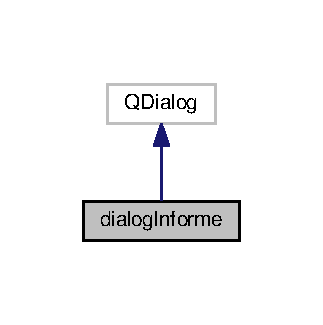
\includegraphics[width=155pt]{classdialogInforme__inherit__graph}
\end{center}
\end{figure}


Collaboration diagram for dialog\+Informe\+:
\nopagebreak
\begin{figure}[H]
\begin{center}
\leavevmode
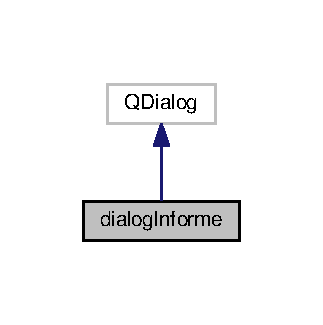
\includegraphics[width=155pt]{classdialogInforme__coll__graph}
\end{center}
\end{figure}
\subsection*{Public Member Functions}
\begin{DoxyCompactItemize}
\item 
\hyperlink{classdialogInforme_a8e040dbe734fc208c6ed0d1dc3c60eab}{dialog\+Informe} (Q\+Widget $\ast$parent=0)
\item 
\hypertarget{classdialogInforme_a4a824cf508e5a604d80238e58fd90712}{}void {\bfseries cargar} (\hyperlink{classpel_1_1Vector}{pel\+::\+Vector}$<$ \hyperlink{classOwner}{Owner} $>$ $\ast$own)\label{classdialogInforme_a4a824cf508e5a604d80238e58fd90712}

\item 
\hypertarget{classdialogInforme_a102b6e99ddd62fabdb95a9600599e7f4}{}void {\bfseries cargar\+H} (\hyperlink{classpel_1_1Vector}{pel\+::\+Vector}$<$ \hyperlink{classentradaHistorial}{entrada\+Historial} $>$ $\ast$his)\label{classdialogInforme_a102b6e99ddd62fabdb95a9600599e7f4}

\item 
\hypertarget{classdialogInforme_a3a5c9e4065f3bab64f8cd5e50fc9703f}{}void {\bfseries quick\+Sort} (\hyperlink{structrank}{rank} arr\mbox{[}$\,$\mbox{]}, int left, int right)\label{classdialogInforme_a3a5c9e4065f3bab64f8cd5e50fc9703f}

\item 
\hypertarget{classdialogInforme_a8a1f96fa6ccf54b1cfd605618e916b9a}{}std\+::string {\bfseries crear\+String} (\hyperlink{classentradaHistorial}{entrada\+Historial} h)\label{classdialogInforme_a8a1f96fa6ccf54b1cfd605618e916b9a}

\item 
\hypertarget{classdialogInforme_adefb1d8af7389ff6aa2f986f6e42d53d}{}void {\bfseries set\+Radio} (int opcion)\label{classdialogInforme_adefb1d8af7389ff6aa2f986f6e42d53d}

\end{DoxyCompactItemize}


\subsection{Constructor \& Destructor Documentation}
\hypertarget{classdialogInforme_a8e040dbe734fc208c6ed0d1dc3c60eab}{}\index{dialog\+Informe@{dialog\+Informe}!dialog\+Informe@{dialog\+Informe}}
\index{dialog\+Informe@{dialog\+Informe}!dialog\+Informe@{dialog\+Informe}}
\subsubsection[{dialog\+Informe}]{\setlength{\rightskip}{0pt plus 5cm}dialog\+Informe\+::dialog\+Informe (
\begin{DoxyParamCaption}
\item[{Q\+Widget $\ast$}]{parent = {\ttfamily 0}}
\end{DoxyParamCaption}
)\hspace{0.3cm}{\ttfamily [explicit]}}\label{classdialogInforme_a8e040dbe734fc208c6ed0d1dc3c60eab}
Copyright 2015 Viaje\+Facil \begin{DoxyAuthor}{Author}
Hugo Ferrando Seage 
\end{DoxyAuthor}


The documentation for this class was generated from the following files\+:\begin{DoxyCompactItemize}
\item 
dialog\+Informe.\+hpp\item 
dialog\+Informe.\+cpp\end{DoxyCompactItemize}

\hypertarget{classdialogLogin}{}\section{dialog\+Login Class Reference}
\label{classdialogLogin}\index{dialog\+Login@{dialog\+Login}}


Dialogo de Usuarios.  




{\ttfamily \#include $<$dialog\+Login.\+hpp$>$}



Inheritance diagram for dialog\+Login\+:
\nopagebreak
\begin{figure}[H]
\begin{center}
\leavevmode
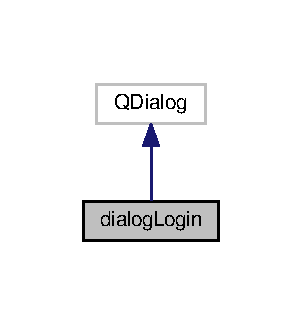
\includegraphics[width=145pt]{classdialogLogin__inherit__graph}
\end{center}
\end{figure}


Collaboration diagram for dialog\+Login\+:
\nopagebreak
\begin{figure}[H]
\begin{center}
\leavevmode
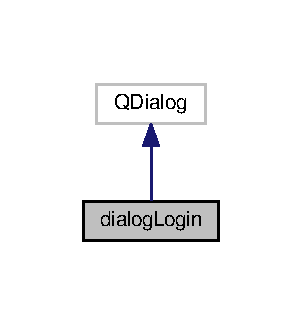
\includegraphics[width=145pt]{classdialogLogin__coll__graph}
\end{center}
\end{figure}
\subsection*{Signals}
\begin{DoxyCompactItemize}
\item 
\hypertarget{classdialogLogin_a051d47d5652799fb46105756e30d60a4}{}void \hyperlink{classdialogLogin_a051d47d5652799fb46105756e30d60a4}{cambio\+De\+Usuario} (std\+::string)\label{classdialogLogin_a051d47d5652799fb46105756e30d60a4}

\begin{DoxyCompactList}\small\item\em cambio\+De\+Usuario Emite una señal con el nombre del usuario que acaba de hacer login para mostrarse en el \hyperlink{classmainWindow}{main\+Window} \end{DoxyCompactList}\end{DoxyCompactItemize}
\subsection*{Public Member Functions}
\begin{DoxyCompactItemize}
\item 
\hyperlink{classdialogLogin_ac2042e079622fb065430200ddba838f1}{dialog\+Login} (Q\+Widget $\ast$parent=0)
\begin{DoxyCompactList}\small\item\em Dialogo de Login Crea y loguea a usuarios. \end{DoxyCompactList}\item 
void \hyperlink{classdialogLogin_ae72837025d8ae73a921ea498d7dceb3b}{set\+Estado} (int estado)
\begin{DoxyCompactList}\small\item\em set\+Estado \end{DoxyCompactList}\end{DoxyCompactItemize}


\subsection{Detailed Description}
Dialogo de Usuarios. 

\subsection{Constructor \& Destructor Documentation}
\hypertarget{classdialogLogin_ac2042e079622fb065430200ddba838f1}{}\index{dialog\+Login@{dialog\+Login}!dialog\+Login@{dialog\+Login}}
\index{dialog\+Login@{dialog\+Login}!dialog\+Login@{dialog\+Login}}
\subsubsection[{dialog\+Login}]{\setlength{\rightskip}{0pt plus 5cm}dialog\+Login\+::dialog\+Login (
\begin{DoxyParamCaption}
\item[{Q\+Widget $\ast$}]{parent = {\ttfamily 0}}
\end{DoxyParamCaption}
)\hspace{0.3cm}{\ttfamily [explicit]}}\label{classdialogLogin_ac2042e079622fb065430200ddba838f1}


Dialogo de Login Crea y loguea a usuarios. 

Copyright 2015 Viaje\+Facil \begin{DoxyAuthor}{Author}
Hugo Ferrando Seage 
\end{DoxyAuthor}


\subsection{Member Function Documentation}
\hypertarget{classdialogLogin_ae72837025d8ae73a921ea498d7dceb3b}{}\index{dialog\+Login@{dialog\+Login}!set\+Estado@{set\+Estado}}
\index{set\+Estado@{set\+Estado}!dialog\+Login@{dialog\+Login}}
\subsubsection[{set\+Estado}]{\setlength{\rightskip}{0pt plus 5cm}void dialog\+Login\+::set\+Estado (
\begin{DoxyParamCaption}
\item[{int}]{estado}
\end{DoxyParamCaption}
)}\label{classdialogLogin_ae72837025d8ae73a921ea498d7dceb3b}


set\+Estado 


\begin{DoxyParams}{Parameters}
{\em estado} & Decide si la ventana se usará para crear un usuario o para hacer login \\
\hline
\end{DoxyParams}


The documentation for this class was generated from the following files\+:\begin{DoxyCompactItemize}
\item 
dialog\+Login.\+hpp\item 
dialog\+Login.\+cpp\end{DoxyCompactItemize}

\hypertarget{classdialogNego}{}\section{dialog\+Nego Class Reference}
\label{classdialogNego}\index{dialog\+Nego@{dialog\+Nego}}


Dialogo de Negos.  




{\ttfamily \#include $<$dialog\+Nego.\+hpp$>$}



Inheritance diagram for dialog\+Nego\+:
\nopagebreak
\begin{figure}[H]
\begin{center}
\leavevmode
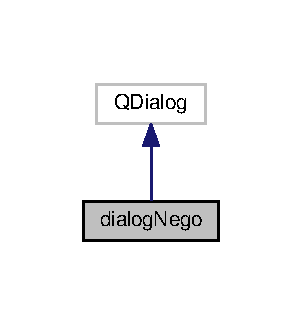
\includegraphics[width=145pt]{classdialogNego__inherit__graph}
\end{center}
\end{figure}


Collaboration diagram for dialog\+Nego\+:
\nopagebreak
\begin{figure}[H]
\begin{center}
\leavevmode
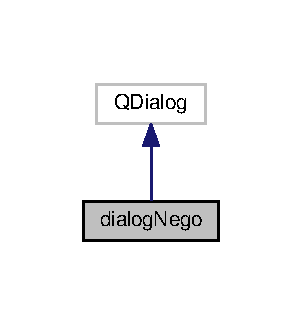
\includegraphics[width=145pt]{classdialogNego__coll__graph}
\end{center}
\end{figure}
\subsection*{Public Member Functions}
\begin{DoxyCompactItemize}
\item 
\hyperlink{classdialogNego_ab093ca8a15c030021d87c540bc5d4da1}{dialog\+Nego} (Q\+Widget $\ast$parent=0)
\item 
void \hyperlink{classdialogNego_a6d97c6b5dcaa5ce2dc283ef4c1514257}{cargar} (\hyperlink{classpel_1_1Vector}{pel\+::\+Vector}$<$ \hyperlink{classOwner}{Owner} $>$ $\ast$own)
\begin{DoxyCompactList}\small\item\em Carga los combo\+Box Recorre el Vector de Owners y rellena el combo\+Box. \end{DoxyCompactList}\item 
void \hyperlink{classdialogNego_a658d77039ffbb8874e8d25af7b00f489}{set\+Nego\+A\+Editar} (\hyperlink{classNego}{Nego} $\ast$neg)
\begin{DoxyCompactList}\small\item\em Edita el \hyperlink{classNego}{Nego} Edita el \hyperlink{classNego}{Nego} que ha sido pasado por referencia. \end{DoxyCompactList}\item 
\hyperlink{classNego}{Nego} \hyperlink{classdialogNego_a525e03d9c16ab7fd99c0bb2476a89b85}{crear} ()
\begin{DoxyCompactList}\small\item\em Crea un \hyperlink{classNego}{Nego} Crea un nuevo \hyperlink{classNego}{Nego} y se lo devuelve a \hyperlink{classmainWindow}{main\+Window}, el cual lo mete en su Vector correspondiente. \end{DoxyCompactList}\item 
int \hyperlink{classdialogNego_a3286fa0d71e65d2b7863d9c32a4787f3}{nivel} ()
\begin{DoxyCompactList}\small\item\em \hyperlink{classOwner}{Owner} seleccionado Devuelve el nivel del combo\+Box. Este nivel indica que \hyperlink{classOwner}{Owner} ha sido seleccionado. Se pasa al \hyperlink{classmainWindow}{main\+Window} para que sepa en que \hyperlink{classOwner}{Owner} tiene que insertar el \hyperlink{classNego}{Nego}. \end{DoxyCompactList}\end{DoxyCompactItemize}


\subsection{Detailed Description}
Dialogo de Negos. 

\subsection{Constructor \& Destructor Documentation}
\hypertarget{classdialogNego_ab093ca8a15c030021d87c540bc5d4da1}{}\index{dialog\+Nego@{dialog\+Nego}!dialog\+Nego@{dialog\+Nego}}
\index{dialog\+Nego@{dialog\+Nego}!dialog\+Nego@{dialog\+Nego}}
\subsubsection[{dialog\+Nego}]{\setlength{\rightskip}{0pt plus 5cm}dialog\+Nego\+::dialog\+Nego (
\begin{DoxyParamCaption}
\item[{Q\+Widget $\ast$}]{parent = {\ttfamily 0}}
\end{DoxyParamCaption}
)\hspace{0.3cm}{\ttfamily [explicit]}}\label{classdialogNego_ab093ca8a15c030021d87c540bc5d4da1}
Copyright 2015 Viaje\+Facil \begin{DoxyAuthor}{Author}
Hugo Ferrando Seage 

David Jiménez Cuevas 

Estefanía Ortego García Se definen las funciones de la ventana grafica \hyperlink{classdialogNego}{dialog\+Nego}, se muestra qué hará cada botón o campo que aparezca (en la ventana gráfica). 
\end{DoxyAuthor}


\subsection{Member Function Documentation}
\hypertarget{classdialogNego_a6d97c6b5dcaa5ce2dc283ef4c1514257}{}\index{dialog\+Nego@{dialog\+Nego}!cargar@{cargar}}
\index{cargar@{cargar}!dialog\+Nego@{dialog\+Nego}}
\subsubsection[{cargar}]{\setlength{\rightskip}{0pt plus 5cm}void dialog\+Nego\+::cargar (
\begin{DoxyParamCaption}
\item[{{\bf pel\+::\+Vector}$<$ {\bf Owner} $>$ $\ast$}]{own}
\end{DoxyParamCaption}
)}\label{classdialogNego_a6d97c6b5dcaa5ce2dc283ef4c1514257}


Carga los combo\+Box Recorre el Vector de Owners y rellena el combo\+Box. 

\hyperlink{classdialogNego_a6d97c6b5dcaa5ce2dc283ef4c1514257}{dialog\+Nego\+::cargar} Carga el combo\+Box con los Owners \hypertarget{classdialogNego_a525e03d9c16ab7fd99c0bb2476a89b85}{}\index{dialog\+Nego@{dialog\+Nego}!crear@{crear}}
\index{crear@{crear}!dialog\+Nego@{dialog\+Nego}}
\subsubsection[{crear}]{\setlength{\rightskip}{0pt plus 5cm}{\bf Nego} dialog\+Nego\+::crear (
\begin{DoxyParamCaption}
{}
\end{DoxyParamCaption}
)}\label{classdialogNego_a525e03d9c16ab7fd99c0bb2476a89b85}


Crea un \hyperlink{classNego}{Nego} Crea un nuevo \hyperlink{classNego}{Nego} y se lo devuelve a \hyperlink{classmainWindow}{main\+Window}, el cual lo mete en su Vector correspondiente. 

Crear un nuevo \hyperlink{classNego}{Nego} Creamos un \hyperlink{classNego}{Nego} con los campos que ha rellenado el usuario. El \hyperlink{classmainWindow}{main\+Window} se encargará de meterlo en el Vector. \hypertarget{classdialogNego_a3286fa0d71e65d2b7863d9c32a4787f3}{}\index{dialog\+Nego@{dialog\+Nego}!nivel@{nivel}}
\index{nivel@{nivel}!dialog\+Nego@{dialog\+Nego}}
\subsubsection[{nivel}]{\setlength{\rightskip}{0pt plus 5cm}int dialog\+Nego\+::nivel (
\begin{DoxyParamCaption}
{}
\end{DoxyParamCaption}
)}\label{classdialogNego_a3286fa0d71e65d2b7863d9c32a4787f3}


\hyperlink{classOwner}{Owner} seleccionado Devuelve el nivel del combo\+Box. Este nivel indica que \hyperlink{classOwner}{Owner} ha sido seleccionado. Se pasa al \hyperlink{classmainWindow}{main\+Window} para que sepa en que \hyperlink{classOwner}{Owner} tiene que insertar el \hyperlink{classNego}{Nego}. 

Devolver el \hyperlink{classOwner}{Owner} seleccionado Devolvemos el índice del \hyperlink{classOwner}{Owner} seleccionado para que el \hyperlink{classmainWindow}{main\+Window} sepa en que Vector de Owners debe meter el nuevo \hyperlink{classNego}{Nego}. \hypertarget{classdialogNego_a658d77039ffbb8874e8d25af7b00f489}{}\index{dialog\+Nego@{dialog\+Nego}!set\+Nego\+A\+Editar@{set\+Nego\+A\+Editar}}
\index{set\+Nego\+A\+Editar@{set\+Nego\+A\+Editar}!dialog\+Nego@{dialog\+Nego}}
\subsubsection[{set\+Nego\+A\+Editar}]{\setlength{\rightskip}{0pt plus 5cm}void dialog\+Nego\+::set\+Nego\+A\+Editar (
\begin{DoxyParamCaption}
\item[{{\bf Nego} $\ast$}]{neg}
\end{DoxyParamCaption}
)}\label{classdialogNego_a658d77039ffbb8874e8d25af7b00f489}


Edita el \hyperlink{classNego}{Nego} Edita el \hyperlink{classNego}{Nego} que ha sido pasado por referencia. 

Preparar la ventana para editar Rellenamos los campos con la referencia del \hyperlink{classOwner}{Owner} pasada, y activamos el flag de editar. 

The documentation for this class was generated from the following files\+:\begin{DoxyCompactItemize}
\item 
dialog\+Nego.\+hpp\item 
dialog\+Nego.\+cpp\end{DoxyCompactItemize}

\hypertarget{classdialogOficinas}{}\section{dialog\+Oficinas Class Reference}
\label{classdialogOficinas}\index{dialog\+Oficinas@{dialog\+Oficinas}}


Inheritance diagram for dialog\+Oficinas\+:
\nopagebreak
\begin{figure}[H]
\begin{center}
\leavevmode
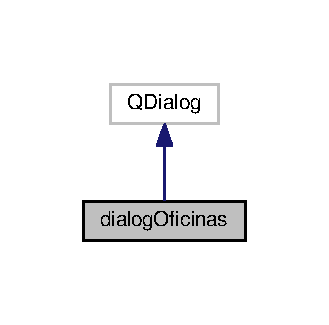
\includegraphics[width=158pt]{classdialogOficinas__inherit__graph}
\end{center}
\end{figure}


Collaboration diagram for dialog\+Oficinas\+:
\nopagebreak
\begin{figure}[H]
\begin{center}
\leavevmode
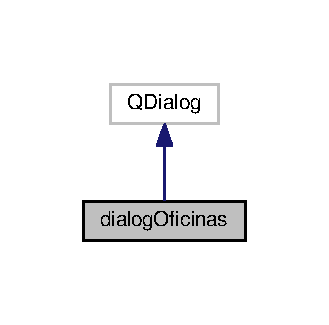
\includegraphics[width=158pt]{classdialogOficinas__coll__graph}
\end{center}
\end{figure}
\subsection*{Public Member Functions}
\begin{DoxyCompactItemize}
\item 
\hypertarget{classdialogOficinas_a38eadc87eb5381d6447af6b54d73bf53}{}{\bfseries dialog\+Oficinas} (Q\+Widget $\ast$parent=0)\label{classdialogOficinas_a38eadc87eb5381d6447af6b54d73bf53}

\item 
\hypertarget{classdialogOficinas_abe9f02cd44d4238b7b68ebd5b029a507}{}void {\bfseries set\+Of} (\hyperlink{classpel_1_1vector}{pel\+::vector}$<$ \hyperlink{classOficina}{Oficina} $>$ $\ast$ofc)\label{classdialogOficinas_abe9f02cd44d4238b7b68ebd5b029a507}

\item 
\hypertarget{classdialogOficinas_a7b129b6519609a19d98dba1353eb4356}{}void {\bfseries set\+Ow} (\hyperlink{classpel_1_1vector}{pel\+::vector}$<$ \hyperlink{classOwner}{Owner} $>$ $\ast$own)\label{classdialogOficinas_a7b129b6519609a19d98dba1353eb4356}

\item 
\hypertarget{classdialogOficinas_af8d8a489575cb71d83c36c6667471aa7}{}void {\bfseries set\+Pe} (\hyperlink{classpel_1_1vector}{pel\+::vector}$<$ \hyperlink{classPeticion}{Peticion} $>$ $\ast$pet)\label{classdialogOficinas_af8d8a489575cb71d83c36c6667471aa7}

\item 
\hypertarget{classdialogOficinas_ad22074f104581639754c4eb1703e1da4}{}void {\bfseries cargar} ()\label{classdialogOficinas_ad22074f104581639754c4eb1703e1da4}

\item 
\hypertarget{classdialogOficinas_a616cff0912d89a0c0f5a54078353c8eb}{}void {\bfseries set\+Oficina\+A\+Editar} (\hyperlink{classOficina}{Oficina} \&ofi)\label{classdialogOficinas_a616cff0912d89a0c0f5a54078353c8eb}

\end{DoxyCompactItemize}


The documentation for this class was generated from the following files\+:\begin{DoxyCompactItemize}
\item 
dialog\+Oficinas.\+hpp\item 
dialog\+Oficinas.\+cpp\end{DoxyCompactItemize}

\hypertarget{classdialogOwner}{}\section{dialog\+Owner Class Reference}
\label{classdialogOwner}\index{dialog\+Owner@{dialog\+Owner}}


The \hyperlink{classdialogOwner}{dialog\+Owner} class.  




{\ttfamily \#include $<$dialog\+Owner.\+hpp$>$}



Inheritance diagram for dialog\+Owner\+:
\nopagebreak
\begin{figure}[H]
\begin{center}
\leavevmode
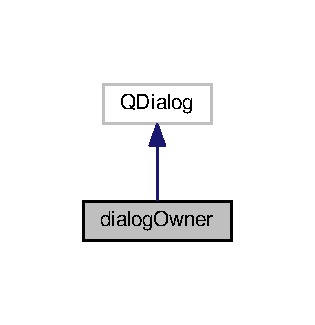
\includegraphics[width=151pt]{classdialogOwner__inherit__graph}
\end{center}
\end{figure}


Collaboration diagram for dialog\+Owner\+:
\nopagebreak
\begin{figure}[H]
\begin{center}
\leavevmode
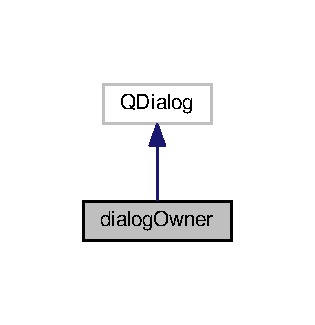
\includegraphics[width=151pt]{classdialogOwner__coll__graph}
\end{center}
\end{figure}
\subsection*{Public Member Functions}
\begin{DoxyCompactItemize}
\item 
\hyperlink{classdialogOwner_a6d4b17329380be5d0a7aa71452e4e0a0}{dialog\+Owner} (Q\+Widget $\ast$parent=0)
\begin{DoxyCompactList}\small\item\em \hyperlink{classdialogOwner}{dialog\+Owner} \end{DoxyCompactList}\item 
\hypertarget{classdialogOwner_adba2ef2a476b1eae66587322fcfac107}{}\hyperlink{classdialogOwner_adba2ef2a476b1eae66587322fcfac107}{$\sim$dialog\+Owner} ()\label{classdialogOwner_adba2ef2a476b1eae66587322fcfac107}

\begin{DoxyCompactList}\small\item\em \hyperlink{classdialogOwner_adba2ef2a476b1eae66587322fcfac107}{dialog\+Owner\+::$\sim$dialog\+Owner} destructor, se destruirán el o los datos seleccionados en owners \end{DoxyCompactList}\item 
void \hyperlink{classdialogOwner_add1764a10a2e39ff76e16cbd19bc1def}{set\+Ow} (\hyperlink{classpel_1_1vector}{pel\+::vector}$<$ \hyperlink{classOwner}{Owner} $>$ $\ast$own)
\begin{DoxyCompactList}\small\item\em set\+Ow \end{DoxyCompactList}\item 
\hypertarget{classdialogOwner_aa91556917f50ed58875fb96b668f6191}{}void {\bfseries set\+Owner\+A\+Editar} (\hyperlink{classOwner}{Owner} \&ow)\label{classdialogOwner_aa91556917f50ed58875fb96b668f6191}

\end{DoxyCompactItemize}


\subsection{Detailed Description}
The \hyperlink{classdialogOwner}{dialog\+Owner} class. 

\subsection{Constructor \& Destructor Documentation}
\hypertarget{classdialogOwner_a6d4b17329380be5d0a7aa71452e4e0a0}{}\index{dialog\+Owner@{dialog\+Owner}!dialog\+Owner@{dialog\+Owner}}
\index{dialog\+Owner@{dialog\+Owner}!dialog\+Owner@{dialog\+Owner}}
\subsubsection[{dialog\+Owner}]{\setlength{\rightskip}{0pt plus 5cm}dialog\+Owner\+::dialog\+Owner (
\begin{DoxyParamCaption}
\item[{Q\+Widget $\ast$}]{parent = {\ttfamily 0}}
\end{DoxyParamCaption}
)\hspace{0.3cm}{\ttfamily [explicit]}}\label{classdialogOwner_a6d4b17329380be5d0a7aa71452e4e0a0}


\hyperlink{classdialogOwner}{dialog\+Owner} 

\hyperlink{classdialogOwner_a6d4b17329380be5d0a7aa71452e4e0a0}{dialog\+Owner\+::dialog\+Owner}


\begin{DoxyParams}{Parameters}
{\em parent} & \\
\hline
{\em parent} & tipo de funcion del dialog owner \\
\hline
\end{DoxyParams}


\subsection{Member Function Documentation}
\hypertarget{classdialogOwner_add1764a10a2e39ff76e16cbd19bc1def}{}\index{dialog\+Owner@{dialog\+Owner}!set\+Ow@{set\+Ow}}
\index{set\+Ow@{set\+Ow}!dialog\+Owner@{dialog\+Owner}}
\subsubsection[{set\+Ow}]{\setlength{\rightskip}{0pt plus 5cm}void dialog\+Owner\+::set\+Ow (
\begin{DoxyParamCaption}
\item[{{\bf pel\+::vector}$<$ {\bf Owner} $>$ $\ast$}]{own}
\end{DoxyParamCaption}
)}\label{classdialogOwner_add1764a10a2e39ff76e16cbd19bc1def}


set\+Ow 

\hyperlink{classdialogOwner_add1764a10a2e39ff76e16cbd19bc1def}{dialog\+Owner\+::set\+Ow}


\begin{DoxyParams}{Parameters}
{\em own} & \\
\hline
\end{DoxyParams}


The documentation for this class was generated from the following files\+:\begin{DoxyCompactItemize}
\item 
dialog\+Owner.\+hpp\item 
dialog\+Owner.\+cpp\end{DoxyCompactItemize}

\hypertarget{classdialogPeticiones}{}\section{dialog\+Peticiones Class Reference}
\label{classdialogPeticiones}\index{dialog\+Peticiones@{dialog\+Peticiones}}


The \hyperlink{classdialogPeticiones}{dialog\+Peticiones} class.  




{\ttfamily \#include $<$dialog\+Peticiones.\+hpp$>$}



Inheritance diagram for dialog\+Peticiones\+:
\nopagebreak
\begin{figure}[H]
\begin{center}
\leavevmode
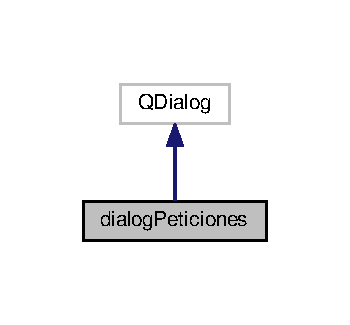
\includegraphics[width=168pt]{classdialogPeticiones__inherit__graph}
\end{center}
\end{figure}


Collaboration diagram for dialog\+Peticiones\+:
\nopagebreak
\begin{figure}[H]
\begin{center}
\leavevmode
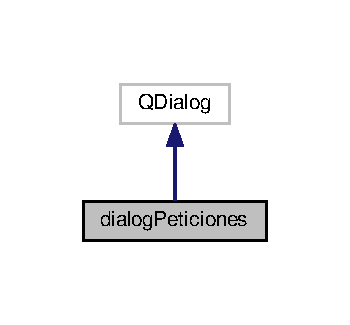
\includegraphics[width=168pt]{classdialogPeticiones__coll__graph}
\end{center}
\end{figure}
\subsection*{Public Member Functions}
\begin{DoxyCompactItemize}
\item 
\hyperlink{classdialogPeticiones_a98d94817a71b0f17a67e4d50e26b0703}{dialog\+Peticiones} (Q\+Widget $\ast$parent=0)
\begin{DoxyCompactList}\small\item\em \hyperlink{classdialogPeticiones}{dialog\+Peticiones} \end{DoxyCompactList}\item 
\hypertarget{classdialogPeticiones_a463f39b52633828f8b8d7047f2770add}{}void \hyperlink{classdialogPeticiones_a463f39b52633828f8b8d7047f2770add}{cargar} (\hyperlink{classpel_1_1Vector}{pel\+::\+Vector}$<$ \hyperlink{classOwner}{Owner} $>$ $\ast$own)\label{classdialogPeticiones_a463f39b52633828f8b8d7047f2770add}

\begin{DoxyCompactList}\small\item\em \hyperlink{classdialogPeticiones_a463f39b52633828f8b8d7047f2770add}{dialog\+Peticiones\+::cargar} \end{DoxyCompactList}\item 
\hypertarget{classdialogPeticiones_a9338b72e5e007b990d8c95a7b12627ea}{}void {\bfseries set\+Peticion\+A\+Editar} (\hyperlink{classPeticion}{Peticion} $\ast$pet)\label{classdialogPeticiones_a9338b72e5e007b990d8c95a7b12627ea}

\item 
\hypertarget{classdialogPeticiones_a3675576259132999c6c52183c7c72bd2}{}\hyperlink{classPeticion}{Peticion} {\bfseries crear} ()\label{classdialogPeticiones_a3675576259132999c6c52183c7c72bd2}

\item 
\hypertarget{classdialogPeticiones_aef911f15aae9cb79ddc92a117dee4f8e}{}int {\bfseries nivel\+Ow} ()\label{classdialogPeticiones_aef911f15aae9cb79ddc92a117dee4f8e}

\item 
\hypertarget{classdialogPeticiones_a18140cebfc622999876f183eb42f6711}{}int {\bfseries nivel\+Of} ()\label{classdialogPeticiones_a18140cebfc622999876f183eb42f6711}

\item 
\hypertarget{classdialogPeticiones_a821022c92ea3a2f543dd0d4bd2916b50}{}int {\bfseries nivel\+Ne} ()\label{classdialogPeticiones_a821022c92ea3a2f543dd0d4bd2916b50}

\end{DoxyCompactItemize}


\subsection{Detailed Description}
The \hyperlink{classdialogPeticiones}{dialog\+Peticiones} class. 

\subsection{Constructor \& Destructor Documentation}
\hypertarget{classdialogPeticiones_a98d94817a71b0f17a67e4d50e26b0703}{}\index{dialog\+Peticiones@{dialog\+Peticiones}!dialog\+Peticiones@{dialog\+Peticiones}}
\index{dialog\+Peticiones@{dialog\+Peticiones}!dialog\+Peticiones@{dialog\+Peticiones}}
\subsubsection[{dialog\+Peticiones}]{\setlength{\rightskip}{0pt plus 5cm}dialog\+Peticiones\+::dialog\+Peticiones (
\begin{DoxyParamCaption}
\item[{Q\+Widget $\ast$}]{parent = {\ttfamily 0}}
\end{DoxyParamCaption}
)\hspace{0.3cm}{\ttfamily [explicit]}}\label{classdialogPeticiones_a98d94817a71b0f17a67e4d50e26b0703}


\hyperlink{classdialogPeticiones}{dialog\+Peticiones} 


\begin{DoxyParams}{Parameters}
{\em parent} & Copyright 2015 Viaje\+Facil \\
\hline
\end{DoxyParams}
\begin{DoxyAuthor}{Author}
Hugo Ferrando Seage 

Sergio Candel 

David Jimenez se tendrá acceso a la cabecera y al cuerpo de \hyperlink{classdialogPeticiones}{dialog\+Peticiones} para usar sus datos 
\end{DoxyAuthor}


The documentation for this class was generated from the following files\+:\begin{DoxyCompactItemize}
\item 
dialog\+Peticiones.\+hpp\item 
dialog\+Peticiones.\+cpp\end{DoxyCompactItemize}

\hypertarget{classentradaHistorial}{}\section{entrada\+Historial Class Reference}
\label{classentradaHistorial}\index{entrada\+Historial@{entrada\+Historial}}


{\ttfamily \#include $<$entrada\+Historial.\+hpp$>$}

\subsection*{Public Member Functions}
\begin{DoxyCompactItemize}
\item 
\hyperlink{classentradaHistorial_a899faea9865c1a89fe24306ce634c646}{entrada\+Historial} ()
\item 
\hypertarget{classentradaHistorial_a481ae6103e351fa708864c5488c4049b}{}{\bfseries entrada\+Historial} (bool c, bool mo, bool bo, std\+::size\+\_\+t as, std\+::string ori, std\+::string des, std\+::string own, std\+::string of, std\+::string pa\+Of, std\+::string co\+Of)\label{classentradaHistorial_a481ae6103e351fa708864c5488c4049b}

\item 
\hypertarget{classentradaHistorial_a3126649df21004164e8ffcb94eedb1ac}{}bool {\bfseries get\+Creado} () const \label{classentradaHistorial_a3126649df21004164e8ffcb94eedb1ac}

\item 
\hypertarget{classentradaHistorial_ae8d5cd603ce4e160a71cde6c0337fa01}{}void {\bfseries set\+Creado} (bool value)\label{classentradaHistorial_ae8d5cd603ce4e160a71cde6c0337fa01}

\item 
\hypertarget{classentradaHistorial_aeb1a67858ec0bdb9b7f388c0add876e5}{}bool {\bfseries get\+Modificado} () const \label{classentradaHistorial_aeb1a67858ec0bdb9b7f388c0add876e5}

\item 
\hypertarget{classentradaHistorial_aab34c7712608b9c2050f057d4fdb8a93}{}void {\bfseries set\+Modificado} (bool value)\label{classentradaHistorial_aab34c7712608b9c2050f057d4fdb8a93}

\item 
\hypertarget{classentradaHistorial_a35f68da05c76c6f05804e5c5b93adbac}{}bool {\bfseries get\+Borrado} () const \label{classentradaHistorial_a35f68da05c76c6f05804e5c5b93adbac}

\item 
\hypertarget{classentradaHistorial_a300ff6824ca98e5ad2c91b9fabd58209}{}void {\bfseries set\+Borrado} (bool value)\label{classentradaHistorial_a300ff6824ca98e5ad2c91b9fabd58209}

\item 
\hypertarget{classentradaHistorial_ad60cb8b617dc385a8abd1c77eb398bfa}{}std\+::size\+\_\+t {\bfseries get\+Asientos} () const \label{classentradaHistorial_ad60cb8b617dc385a8abd1c77eb398bfa}

\item 
\hypertarget{classentradaHistorial_acc13a64252b363eb20f07971bd42c017}{}void {\bfseries set\+Asientos} (std\+::size\+\_\+t value)\label{classentradaHistorial_acc13a64252b363eb20f07971bd42c017}

\item 
\hypertarget{classentradaHistorial_ab5940dd29832022c690592046b6706b5}{}std\+::string {\bfseries get\+Origen} () const \label{classentradaHistorial_ab5940dd29832022c690592046b6706b5}

\item 
\hypertarget{classentradaHistorial_aa47ecc85880e1179101fd49a969f6116}{}void {\bfseries set\+Origen} (const std\+::string \&value)\label{classentradaHistorial_aa47ecc85880e1179101fd49a969f6116}

\item 
\hypertarget{classentradaHistorial_a40949ba76750eb357ed8a1d860ec7842}{}std\+::string {\bfseries get\+Destino} () const \label{classentradaHistorial_a40949ba76750eb357ed8a1d860ec7842}

\item 
\hypertarget{classentradaHistorial_a7142ed9728009f55e5516a1433e324dc}{}void {\bfseries set\+Destino} (const std\+::string \&value)\label{classentradaHistorial_a7142ed9728009f55e5516a1433e324dc}

\item 
\hypertarget{classentradaHistorial_ae95fd866b07baa0bb06ab57acf0dc8c4}{}std\+::string {\bfseries get\+Oficina} () const \label{classentradaHistorial_ae95fd866b07baa0bb06ab57acf0dc8c4}

\item 
\hypertarget{classentradaHistorial_a431df3b322941df18e376022d5d7f89a}{}void {\bfseries set\+Oficina} (const std\+::string \&value)\label{classentradaHistorial_a431df3b322941df18e376022d5d7f89a}

\item 
\hypertarget{classentradaHistorial_aa11f9a3ea0fee9ac8f71a83c5dfa97ed}{}std\+::string {\bfseries get\+Pais\+Oficina} () const \label{classentradaHistorial_aa11f9a3ea0fee9ac8f71a83c5dfa97ed}

\item 
\hypertarget{classentradaHistorial_a7ba50bae0da3388440153d3c8b35863e}{}void {\bfseries set\+Pais\+Oficina} (const std\+::string \&value)\label{classentradaHistorial_a7ba50bae0da3388440153d3c8b35863e}

\item 
\hypertarget{classentradaHistorial_a636f820854ec922bd6fd22e38e5acb84}{}std\+::string {\bfseries get\+Continente\+Oficina} () const \label{classentradaHistorial_a636f820854ec922bd6fd22e38e5acb84}

\item 
\hypertarget{classentradaHistorial_affde03b37e865a5e086c6191b801a1b8}{}void {\bfseries set\+Continente\+Oficina} (const std\+::string \&value)\label{classentradaHistorial_affde03b37e865a5e086c6191b801a1b8}

\item 
\hypertarget{classentradaHistorial_a81bccc82b3b3295ed258eb3923bca2cc}{}std\+::string {\bfseries get\+Owner} () const \label{classentradaHistorial_a81bccc82b3b3295ed258eb3923bca2cc}

\item 
\hypertarget{classentradaHistorial_a876a1124e1ed5294f1bd20be50f54b4d}{}void {\bfseries set\+Owner} (const std\+::string \&value)\label{classentradaHistorial_a876a1124e1ed5294f1bd20be50f54b4d}

\end{DoxyCompactItemize}


\subsection{Detailed Description}
Copyright 2015 Viaje\+Facil \begin{DoxyAuthor}{Author}
Hugo Ferrando Seage 
\end{DoxyAuthor}


\subsection{Constructor \& Destructor Documentation}
\hypertarget{classentradaHistorial_a899faea9865c1a89fe24306ce634c646}{}\index{entrada\+Historial@{entrada\+Historial}!entrada\+Historial@{entrada\+Historial}}
\index{entrada\+Historial@{entrada\+Historial}!entrada\+Historial@{entrada\+Historial}}
\subsubsection[{entrada\+Historial}]{\setlength{\rightskip}{0pt plus 5cm}entrada\+Historial\+::entrada\+Historial (
\begin{DoxyParamCaption}
{}
\end{DoxyParamCaption}
)}\label{classentradaHistorial_a899faea9865c1a89fe24306ce634c646}
Copyright 2015 Viaje\+Facil \begin{DoxyAuthor}{Author}
Hugo Ferrando Seage 
\end{DoxyAuthor}


The documentation for this class was generated from the following files\+:\begin{DoxyCompactItemize}
\item 
entrada\+Historial.\+hpp\item 
entrada\+Historial.\+cpp\end{DoxyCompactItemize}

\hypertarget{classFecha}{}\section{Fecha Class Reference}
\label{classFecha}\index{Fecha@{Fecha}}


The \hyperlink{classFecha}{Fecha} class.  




{\ttfamily \#include $<$fecha.\+hpp$>$}

\subsection*{Public Member Functions}
\begin{DoxyCompactItemize}
\item 
\hyperlink{classFecha_a5fbc6564d9c48e73cf8d27568a2a7fc5}{Fecha} ()
\begin{DoxyCompactList}\small\item\em \hyperlink{classFecha}{Fecha}. \end{DoxyCompactList}\item 
\hyperlink{classFecha_ac4e53e6fcbb50c3619cfc60e1a5de016}{Fecha} (std\+::size\+\_\+t dia, std\+::size\+\_\+t mes, int anio)
\begin{DoxyCompactList}\small\item\em \hyperlink{classFecha}{Fecha}. \end{DoxyCompactList}\item 
\hypertarget{classFecha_ae34f2ebe1ac7f3a78eefb68e8d1c8b86}{}\hyperlink{classFecha_ae34f2ebe1ac7f3a78eefb68e8d1c8b86}{$\sim$\+Fecha} ()\label{classFecha_ae34f2ebe1ac7f3a78eefb68e8d1c8b86}

\begin{DoxyCompactList}\small\item\em \hyperlink{classFecha_ae34f2ebe1ac7f3a78eefb68e8d1c8b86}{Fecha\+::$\sim$\+Fecha}. \end{DoxyCompactList}\item 
void \hyperlink{classFecha_a3040cb959b0b779c262805460d9786bb}{set\+Fecha} (std\+::size\+\_\+t dia, std\+::size\+\_\+t mes, int anio)
\begin{DoxyCompactList}\small\item\em set\+Fecha \end{DoxyCompactList}\item 
void \hyperlink{classFecha_a19af0818e81aa8d74b60fdfca7aabb04}{set\+Dia} (std\+::size\+\_\+t dia)
\begin{DoxyCompactList}\small\item\em set\+Dia \end{DoxyCompactList}\item 
void \hyperlink{classFecha_a0167b058fedd612cd2c29c3d932d0741}{set\+Mes} (std\+::size\+\_\+t mes)
\begin{DoxyCompactList}\small\item\em set\+Mes \end{DoxyCompactList}\item 
void \hyperlink{classFecha_a3cfbea8834e7a23023f11c3d069838f0}{set\+Anio} (int anio)
\begin{DoxyCompactList}\small\item\em set\+Anio \end{DoxyCompactList}\item 
std\+::size\+\_\+t \hyperlink{classFecha_a1a2191fb9b522845f249f5f1af233f58}{get\+Dia} ()
\begin{DoxyCompactList}\small\item\em get\+Dia \end{DoxyCompactList}\item 
std\+::size\+\_\+t \hyperlink{classFecha_adab1b3eed2b3e81ccf7bc78c456635ce}{get\+Mes} ()
\begin{DoxyCompactList}\small\item\em get\+Mes \end{DoxyCompactList}\item 
int \hyperlink{classFecha_a89ebafe74bc6e5f53ad688dce1d3fc26}{get\+Anio} ()
\begin{DoxyCompactList}\small\item\em get\+Anio \end{DoxyCompactList}\item 
{\footnotesize template$<$class Archive $>$ }\\void \hyperlink{classFecha_a8e2b7a6977d7d6354647af025808f750}{serialize} (Archive \&archive)
\begin{DoxyCompactList}\small\item\em serialize \end{DoxyCompactList}\end{DoxyCompactItemize}


\subsection{Detailed Description}
The \hyperlink{classFecha}{Fecha} class. 

\subsection{Constructor \& Destructor Documentation}
\hypertarget{classFecha_a5fbc6564d9c48e73cf8d27568a2a7fc5}{}\index{Fecha@{Fecha}!Fecha@{Fecha}}
\index{Fecha@{Fecha}!Fecha@{Fecha}}
\subsubsection[{Fecha}]{\setlength{\rightskip}{0pt plus 5cm}Fecha\+::\+Fecha (
\begin{DoxyParamCaption}
{}
\end{DoxyParamCaption}
)}\label{classFecha_a5fbc6564d9c48e73cf8d27568a2a7fc5}


\hyperlink{classFecha}{Fecha}. 

\hyperlink{classFecha_a5fbc6564d9c48e73cf8d27568a2a7fc5}{Fecha\+::\+Fecha}. \hypertarget{classFecha_ac4e53e6fcbb50c3619cfc60e1a5de016}{}\index{Fecha@{Fecha}!Fecha@{Fecha}}
\index{Fecha@{Fecha}!Fecha@{Fecha}}
\subsubsection[{Fecha}]{\setlength{\rightskip}{0pt plus 5cm}Fecha\+::\+Fecha (
\begin{DoxyParamCaption}
\item[{std\+::size\+\_\+t}]{dia, }
\item[{std\+::size\+\_\+t}]{mes, }
\item[{int}]{anio}
\end{DoxyParamCaption}
)}\label{classFecha_ac4e53e6fcbb50c3619cfc60e1a5de016}


\hyperlink{classFecha}{Fecha}. 


\begin{DoxyParams}{Parameters}
{\em dia} & \\
\hline
{\em mes} & \\
\hline
{\em anio} & \\
\hline
\end{DoxyParams}


\subsection{Member Function Documentation}
\hypertarget{classFecha_a89ebafe74bc6e5f53ad688dce1d3fc26}{}\index{Fecha@{Fecha}!get\+Anio@{get\+Anio}}
\index{get\+Anio@{get\+Anio}!Fecha@{Fecha}}
\subsubsection[{get\+Anio}]{\setlength{\rightskip}{0pt plus 5cm}int Fecha\+::get\+Anio (
\begin{DoxyParamCaption}
{}
\end{DoxyParamCaption}
)}\label{classFecha_a89ebafe74bc6e5f53ad688dce1d3fc26}


get\+Anio 

\hyperlink{classFecha_a89ebafe74bc6e5f53ad688dce1d3fc26}{Fecha\+::get\+Anio}.

\begin{DoxyReturn}{Returns}

\end{DoxyReturn}
\hypertarget{classFecha_a1a2191fb9b522845f249f5f1af233f58}{}\index{Fecha@{Fecha}!get\+Dia@{get\+Dia}}
\index{get\+Dia@{get\+Dia}!Fecha@{Fecha}}
\subsubsection[{get\+Dia}]{\setlength{\rightskip}{0pt plus 5cm}size\+\_\+t Fecha\+::get\+Dia (
\begin{DoxyParamCaption}
{}
\end{DoxyParamCaption}
)}\label{classFecha_a1a2191fb9b522845f249f5f1af233f58}


get\+Dia 

\hyperlink{classFecha_a1a2191fb9b522845f249f5f1af233f58}{Fecha\+::get\+Dia}.

\begin{DoxyReturn}{Returns}

\end{DoxyReturn}
\hypertarget{classFecha_adab1b3eed2b3e81ccf7bc78c456635ce}{}\index{Fecha@{Fecha}!get\+Mes@{get\+Mes}}
\index{get\+Mes@{get\+Mes}!Fecha@{Fecha}}
\subsubsection[{get\+Mes}]{\setlength{\rightskip}{0pt plus 5cm}size\+\_\+t Fecha\+::get\+Mes (
\begin{DoxyParamCaption}
{}
\end{DoxyParamCaption}
)}\label{classFecha_adab1b3eed2b3e81ccf7bc78c456635ce}


get\+Mes 

\hyperlink{classFecha_adab1b3eed2b3e81ccf7bc78c456635ce}{Fecha\+::get\+Mes}.

\begin{DoxyReturn}{Returns}

\end{DoxyReturn}
\hypertarget{classFecha_a8e2b7a6977d7d6354647af025808f750}{}\index{Fecha@{Fecha}!serialize@{serialize}}
\index{serialize@{serialize}!Fecha@{Fecha}}
\subsubsection[{serialize}]{\setlength{\rightskip}{0pt plus 5cm}template$<$class Archive $>$ void Fecha\+::serialize (
\begin{DoxyParamCaption}
\item[{Archive \&}]{archive}
\end{DoxyParamCaption}
)\hspace{0.3cm}{\ttfamily [inline]}}\label{classFecha_a8e2b7a6977d7d6354647af025808f750}


serialize 


\begin{DoxyParams}{Parameters}
{\em archive} & \\
\hline
\end{DoxyParams}
archive

cereal\+::make\+\_\+nvp\hypertarget{classFecha_a3cfbea8834e7a23023f11c3d069838f0}{}\index{Fecha@{Fecha}!set\+Anio@{set\+Anio}}
\index{set\+Anio@{set\+Anio}!Fecha@{Fecha}}
\subsubsection[{set\+Anio}]{\setlength{\rightskip}{0pt plus 5cm}void Fecha\+::set\+Anio (
\begin{DoxyParamCaption}
\item[{int}]{anio}
\end{DoxyParamCaption}
)}\label{classFecha_a3cfbea8834e7a23023f11c3d069838f0}


set\+Anio 

\hyperlink{classFecha_a3cfbea8834e7a23023f11c3d069838f0}{Fecha\+::set\+Anio}.


\begin{DoxyParams}{Parameters}
{\em anio} & \\
\hline
\end{DoxyParams}
\hypertarget{classFecha_a19af0818e81aa8d74b60fdfca7aabb04}{}\index{Fecha@{Fecha}!set\+Dia@{set\+Dia}}
\index{set\+Dia@{set\+Dia}!Fecha@{Fecha}}
\subsubsection[{set\+Dia}]{\setlength{\rightskip}{0pt plus 5cm}void Fecha\+::set\+Dia (
\begin{DoxyParamCaption}
\item[{std\+::size\+\_\+t}]{dia}
\end{DoxyParamCaption}
)}\label{classFecha_a19af0818e81aa8d74b60fdfca7aabb04}


set\+Dia 

\hyperlink{classFecha_a19af0818e81aa8d74b60fdfca7aabb04}{Fecha\+::set\+Dia}.


\begin{DoxyParams}{Parameters}
{\em dia} & set\+Dia \\
\hline
{\em dia} & \\
\hline
{\em dia} & \\
\hline
\end{DoxyParams}
\hypertarget{classFecha_a3040cb959b0b779c262805460d9786bb}{}\index{Fecha@{Fecha}!set\+Fecha@{set\+Fecha}}
\index{set\+Fecha@{set\+Fecha}!Fecha@{Fecha}}
\subsubsection[{set\+Fecha}]{\setlength{\rightskip}{0pt plus 5cm}void Fecha\+::set\+Fecha (
\begin{DoxyParamCaption}
\item[{std\+::size\+\_\+t}]{dia, }
\item[{std\+::size\+\_\+t}]{mes, }
\item[{int}]{anio}
\end{DoxyParamCaption}
)}\label{classFecha_a3040cb959b0b779c262805460d9786bb}


set\+Fecha 

\hyperlink{classFecha_a3040cb959b0b779c262805460d9786bb}{Fecha\+::set\+Fecha}.


\begin{DoxyParams}{Parameters}
{\em dia} & \\
\hline
{\em mes} & \\
\hline
{\em anio} & \\
\hline
\end{DoxyParams}
\hypertarget{classFecha_a0167b058fedd612cd2c29c3d932d0741}{}\index{Fecha@{Fecha}!set\+Mes@{set\+Mes}}
\index{set\+Mes@{set\+Mes}!Fecha@{Fecha}}
\subsubsection[{set\+Mes}]{\setlength{\rightskip}{0pt plus 5cm}void Fecha\+::set\+Mes (
\begin{DoxyParamCaption}
\item[{std\+::size\+\_\+t}]{mes}
\end{DoxyParamCaption}
)}\label{classFecha_a0167b058fedd612cd2c29c3d932d0741}


set\+Mes 

\hyperlink{classFecha_a0167b058fedd612cd2c29c3d932d0741}{Fecha\+::set\+Mes}.


\begin{DoxyParams}{Parameters}
{\em mes} & \\
\hline
\end{DoxyParams}


The documentation for this class was generated from the following files\+:\begin{DoxyCompactItemize}
\item 
fecha.\+hpp\item 
fecha.\+cpp\end{DoxyCompactItemize}

\hypertarget{classmainWindow}{}\section{main\+Window Class Reference}
\label{classmainWindow}\index{main\+Window@{main\+Window}}


The \hyperlink{classmainWindow}{main\+Window} class.  




{\ttfamily \#include $<$main\+Window.\+hpp$>$}



Inheritance diagram for main\+Window\+:
\nopagebreak
\begin{figure}[H]
\begin{center}
\leavevmode
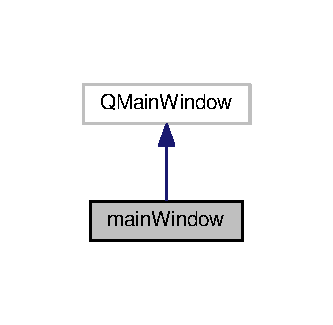
\includegraphics[width=160pt]{classmainWindow__inherit__graph}
\end{center}
\end{figure}


Collaboration diagram for main\+Window\+:
\nopagebreak
\begin{figure}[H]
\begin{center}
\leavevmode
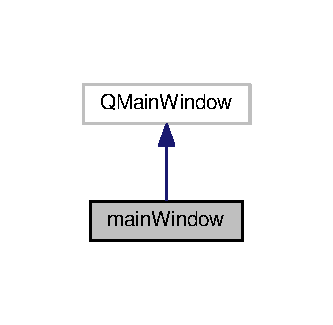
\includegraphics[width=160pt]{classmainWindow__coll__graph}
\end{center}
\end{figure}
\subsection*{Public Member Functions}
\begin{DoxyCompactItemize}
\item 
\hyperlink{classmainWindow_a2c09a8baf94af0cc5109fcf2ef97b12a}{main\+Window} (Q\+Widget $\ast$parent=0)
\begin{DoxyCompactList}\small\item\em \hyperlink{classmainWindow}{main\+Window} \end{DoxyCompactList}\item 
\hypertarget{classmainWindow_a2c4caa71599521dbde5bc35b230ed648}{}\hyperlink{classmainWindow_a2c4caa71599521dbde5bc35b230ed648}{$\sim$main\+Window} ()\label{classmainWindow_a2c4caa71599521dbde5bc35b230ed648}

\begin{DoxyCompactList}\small\item\em \hyperlink{classmainWindow_a2c4caa71599521dbde5bc35b230ed648}{main\+Window\+::$\sim$main\+Window} \end{DoxyCompactList}\end{DoxyCompactItemize}


\subsection{Detailed Description}
The \hyperlink{classmainWindow}{main\+Window} class. 

\subsection{Constructor \& Destructor Documentation}
\hypertarget{classmainWindow_a2c09a8baf94af0cc5109fcf2ef97b12a}{}\index{main\+Window@{main\+Window}!main\+Window@{main\+Window}}
\index{main\+Window@{main\+Window}!main\+Window@{main\+Window}}
\subsubsection[{main\+Window}]{\setlength{\rightskip}{0pt plus 5cm}main\+Window\+::main\+Window (
\begin{DoxyParamCaption}
\item[{Q\+Widget $\ast$}]{parent = {\ttfamily 0}}
\end{DoxyParamCaption}
)\hspace{0.3cm}{\ttfamily [explicit]}}\label{classmainWindow_a2c09a8baf94af0cc5109fcf2ef97b12a}


\hyperlink{classmainWindow}{main\+Window} 

\hyperlink{classmainWindow_a2c09a8baf94af0cc5109fcf2ef97b12a}{main\+Window\+::main\+Window}


\begin{DoxyParams}{Parameters}
{\em parent} & \\
\hline
\end{DoxyParams}


The documentation for this class was generated from the following files\+:\begin{DoxyCompactItemize}
\item 
main\+Window.\+hpp\item 
main\+Window.\+cpp\end{DoxyCompactItemize}

\hypertarget{classNego}{}\section{Nego Class Reference}
\label{classNego}\index{Nego@{Nego}}


The \hyperlink{classNego}{Nego} class.  




{\ttfamily \#include $<$nego.\+hpp$>$}

\subsection*{Public Member Functions}
\begin{DoxyCompactItemize}
\item 
\hyperlink{classNego_af997efc08cdc4e0fc654e6294ac4b08b}{Nego} ()
\begin{DoxyCompactList}\small\item\em \hyperlink{classNego}{Nego}. \end{DoxyCompactList}\item 
\hyperlink{classNego_a612bceb68453277f47491aa2cdaf0963}{Nego} (std\+::string origen, std\+::string destino, int numero\+Plazas, \hyperlink{classFecha}{Fecha} fecha)
\begin{DoxyCompactList}\small\item\em \hyperlink{classNego}{Nego}. \end{DoxyCompactList}\item 
\hypertarget{classNego_af7be4e019e1aa8aaae080e9900574c74}{}\hyperlink{classNego_af7be4e019e1aa8aaae080e9900574c74}{$\sim$\+Nego} ()\label{classNego_af7be4e019e1aa8aaae080e9900574c74}

\begin{DoxyCompactList}\small\item\em \hyperlink{classNego_af7be4e019e1aa8aaae080e9900574c74}{Nego\+::$\sim$\+Nego}. \end{DoxyCompactList}\item 
void \hyperlink{classNego_a886d652e1dd9f66c387978dbbcbf6aec}{set\+Nego} (std\+::string origen, std\+::string destino, int numero\+Plazas, \hyperlink{classFecha}{Fecha} fecha)
\begin{DoxyCompactList}\small\item\em set\+Nego \end{DoxyCompactList}\item 
void \hyperlink{classNego_ab9a55ac4fb4834dbede2806dbbcb62bb}{set\+Origen} (std\+::string origen)
\begin{DoxyCompactList}\small\item\em set\+Origen \end{DoxyCompactList}\item 
void \hyperlink{classNego_a037842afd947e4f33de78ecb4ce0485c}{set\+Destino} (std\+::string destino)
\begin{DoxyCompactList}\small\item\em set\+Destino \end{DoxyCompactList}\item 
void \hyperlink{classNego_ad3b026b1faf221046acb58ee10906ec8}{set\+Numero\+Plazas} (int numero\+Plazas)
\begin{DoxyCompactList}\small\item\em set\+Numero\+Plazas \end{DoxyCompactList}\item 
void \hyperlink{classNego_a8fd1c05283f046daab60ed330bac1795}{set\+Fecha} (\hyperlink{classFecha}{Fecha} fecha)
\begin{DoxyCompactList}\small\item\em set\+Fecha \end{DoxyCompactList}\item 
std\+::string \hyperlink{classNego_a6be2088a392ae71ae25ff281e8432cc3}{get\+Origen} ()
\begin{DoxyCompactList}\small\item\em get\+Origen \end{DoxyCompactList}\item 
std\+::string \hyperlink{classNego_ade01b1e886a2b8e68152338a0ffd1240}{get\+Destino} ()
\begin{DoxyCompactList}\small\item\em get\+Destino \end{DoxyCompactList}\item 
int \hyperlink{classNego_a28cd95d6e56112d813e2128d553cdae7}{get\+Numero\+Plazas} ()
\begin{DoxyCompactList}\small\item\em get\+Numero\+Plazas \end{DoxyCompactList}\item 
\hyperlink{classFecha}{Fecha} \hyperlink{classNego_a83559824f47d518d3bb70d260262d676}{get\+Fecha} ()
\begin{DoxyCompactList}\small\item\em get\+Fecha \end{DoxyCompactList}\item 
{\footnotesize template$<$class Archive $>$ }\\void \hyperlink{classNego_af2aa46474903fc02942fa44d4576fcad}{serialize} (Archive \&archive)
\begin{DoxyCompactList}\small\item\em serialize \end{DoxyCompactList}\end{DoxyCompactItemize}


\subsection{Detailed Description}
The \hyperlink{classNego}{Nego} class. 

\subsection{Constructor \& Destructor Documentation}
\hypertarget{classNego_af997efc08cdc4e0fc654e6294ac4b08b}{}\index{Nego@{Nego}!Nego@{Nego}}
\index{Nego@{Nego}!Nego@{Nego}}
\subsubsection[{Nego}]{\setlength{\rightskip}{0pt plus 5cm}Nego\+::\+Nego (
\begin{DoxyParamCaption}
{}
\end{DoxyParamCaption}
)}\label{classNego_af997efc08cdc4e0fc654e6294ac4b08b}


\hyperlink{classNego}{Nego}. 

\hyperlink{classNego_af997efc08cdc4e0fc654e6294ac4b08b}{Nego\+::\+Nego}. \hypertarget{classNego_a612bceb68453277f47491aa2cdaf0963}{}\index{Nego@{Nego}!Nego@{Nego}}
\index{Nego@{Nego}!Nego@{Nego}}
\subsubsection[{Nego}]{\setlength{\rightskip}{0pt plus 5cm}Nego\+::\+Nego (
\begin{DoxyParamCaption}
\item[{std\+::string}]{origen, }
\item[{std\+::string}]{destino, }
\item[{int}]{numero\+Plazas, }
\item[{{\bf Fecha}}]{fecha}
\end{DoxyParamCaption}
)}\label{classNego_a612bceb68453277f47491aa2cdaf0963}


\hyperlink{classNego}{Nego}. 

\hyperlink{classNego_af997efc08cdc4e0fc654e6294ac4b08b}{Nego\+::\+Nego}.


\begin{DoxyParams}{Parameters}
{\em origen} & \\
\hline
{\em destino} & \\
\hline
{\em numero\+Plazas} & \\
\hline
{\em fecha} & \\
\hline
\end{DoxyParams}


\subsection{Member Function Documentation}
\hypertarget{classNego_ade01b1e886a2b8e68152338a0ffd1240}{}\index{Nego@{Nego}!get\+Destino@{get\+Destino}}
\index{get\+Destino@{get\+Destino}!Nego@{Nego}}
\subsubsection[{get\+Destino}]{\setlength{\rightskip}{0pt plus 5cm}std\+::string Nego\+::get\+Destino (
\begin{DoxyParamCaption}
{}
\end{DoxyParamCaption}
)}\label{classNego_ade01b1e886a2b8e68152338a0ffd1240}


get\+Destino 

\hyperlink{classNego_ade01b1e886a2b8e68152338a0ffd1240}{Nego\+::get\+Destino}.

\begin{DoxyReturn}{Returns}

\end{DoxyReturn}
\hypertarget{classNego_a83559824f47d518d3bb70d260262d676}{}\index{Nego@{Nego}!get\+Fecha@{get\+Fecha}}
\index{get\+Fecha@{get\+Fecha}!Nego@{Nego}}
\subsubsection[{get\+Fecha}]{\setlength{\rightskip}{0pt plus 5cm}{\bf Fecha} Nego\+::get\+Fecha (
\begin{DoxyParamCaption}
{}
\end{DoxyParamCaption}
)}\label{classNego_a83559824f47d518d3bb70d260262d676}


get\+Fecha 

\hyperlink{classNego_a83559824f47d518d3bb70d260262d676}{Nego\+::get\+Fecha}.

\begin{DoxyReturn}{Returns}

\end{DoxyReturn}
\hypertarget{classNego_a28cd95d6e56112d813e2128d553cdae7}{}\index{Nego@{Nego}!get\+Numero\+Plazas@{get\+Numero\+Plazas}}
\index{get\+Numero\+Plazas@{get\+Numero\+Plazas}!Nego@{Nego}}
\subsubsection[{get\+Numero\+Plazas}]{\setlength{\rightskip}{0pt plus 5cm}int Nego\+::get\+Numero\+Plazas (
\begin{DoxyParamCaption}
{}
\end{DoxyParamCaption}
)}\label{classNego_a28cd95d6e56112d813e2128d553cdae7}


get\+Numero\+Plazas 

\hyperlink{classNego_a28cd95d6e56112d813e2128d553cdae7}{Nego\+::get\+Numero\+Plazas}.

\begin{DoxyReturn}{Returns}

\end{DoxyReturn}
\hypertarget{classNego_a6be2088a392ae71ae25ff281e8432cc3}{}\index{Nego@{Nego}!get\+Origen@{get\+Origen}}
\index{get\+Origen@{get\+Origen}!Nego@{Nego}}
\subsubsection[{get\+Origen}]{\setlength{\rightskip}{0pt plus 5cm}std\+::string Nego\+::get\+Origen (
\begin{DoxyParamCaption}
{}
\end{DoxyParamCaption}
)}\label{classNego_a6be2088a392ae71ae25ff281e8432cc3}


get\+Origen 

\hyperlink{classNego_a6be2088a392ae71ae25ff281e8432cc3}{Nego\+::get\+Origen}.

\begin{DoxyReturn}{Returns}

\end{DoxyReturn}
\hypertarget{classNego_af2aa46474903fc02942fa44d4576fcad}{}\index{Nego@{Nego}!serialize@{serialize}}
\index{serialize@{serialize}!Nego@{Nego}}
\subsubsection[{serialize}]{\setlength{\rightskip}{0pt plus 5cm}template$<$class Archive $>$ void Nego\+::serialize (
\begin{DoxyParamCaption}
\item[{Archive \&}]{archive}
\end{DoxyParamCaption}
)\hspace{0.3cm}{\ttfamily [inline]}}\label{classNego_af2aa46474903fc02942fa44d4576fcad}


serialize 


\begin{DoxyParams}{Parameters}
{\em archive} & \\
\hline
\end{DoxyParams}
archive

cereal\+::make\+\_\+nvp

cereal\+::make\+\_\+nvp\hypertarget{classNego_a037842afd947e4f33de78ecb4ce0485c}{}\index{Nego@{Nego}!set\+Destino@{set\+Destino}}
\index{set\+Destino@{set\+Destino}!Nego@{Nego}}
\subsubsection[{set\+Destino}]{\setlength{\rightskip}{0pt plus 5cm}void Nego\+::set\+Destino (
\begin{DoxyParamCaption}
\item[{std\+::string}]{destino}
\end{DoxyParamCaption}
)}\label{classNego_a037842afd947e4f33de78ecb4ce0485c}


set\+Destino 

\hyperlink{classNego_a037842afd947e4f33de78ecb4ce0485c}{Nego\+::set\+Destino}.


\begin{DoxyParams}{Parameters}
{\em destino} & \\
\hline
\end{DoxyParams}
\hypertarget{classNego_a8fd1c05283f046daab60ed330bac1795}{}\index{Nego@{Nego}!set\+Fecha@{set\+Fecha}}
\index{set\+Fecha@{set\+Fecha}!Nego@{Nego}}
\subsubsection[{set\+Fecha}]{\setlength{\rightskip}{0pt plus 5cm}void Nego\+::set\+Fecha (
\begin{DoxyParamCaption}
\item[{{\bf Fecha}}]{fecha}
\end{DoxyParamCaption}
)}\label{classNego_a8fd1c05283f046daab60ed330bac1795}


set\+Fecha 

\hyperlink{classNego_a8fd1c05283f046daab60ed330bac1795}{Nego\+::set\+Fecha}.


\begin{DoxyParams}{Parameters}
{\em fecha} & \\
\hline
\end{DoxyParams}
\hypertarget{classNego_a886d652e1dd9f66c387978dbbcbf6aec}{}\index{Nego@{Nego}!set\+Nego@{set\+Nego}}
\index{set\+Nego@{set\+Nego}!Nego@{Nego}}
\subsubsection[{set\+Nego}]{\setlength{\rightskip}{0pt plus 5cm}void Nego\+::set\+Nego (
\begin{DoxyParamCaption}
\item[{std\+::string}]{origen, }
\item[{std\+::string}]{destino, }
\item[{int}]{numero\+Plazas, }
\item[{{\bf Fecha}}]{fecha}
\end{DoxyParamCaption}
)}\label{classNego_a886d652e1dd9f66c387978dbbcbf6aec}


set\+Nego 

\hyperlink{classNego_a886d652e1dd9f66c387978dbbcbf6aec}{Nego\+::set\+Nego}.


\begin{DoxyParams}{Parameters}
{\em origen} & \\
\hline
{\em destino} & \\
\hline
{\em numero\+Plazas} & \\
\hline
{\em fecha} & \\
\hline
\end{DoxyParams}
\hypertarget{classNego_ad3b026b1faf221046acb58ee10906ec8}{}\index{Nego@{Nego}!set\+Numero\+Plazas@{set\+Numero\+Plazas}}
\index{set\+Numero\+Plazas@{set\+Numero\+Plazas}!Nego@{Nego}}
\subsubsection[{set\+Numero\+Plazas}]{\setlength{\rightskip}{0pt plus 5cm}void Nego\+::set\+Numero\+Plazas (
\begin{DoxyParamCaption}
\item[{int}]{numero\+Plazas}
\end{DoxyParamCaption}
)}\label{classNego_ad3b026b1faf221046acb58ee10906ec8}


set\+Numero\+Plazas 

\hyperlink{classNego_ad3b026b1faf221046acb58ee10906ec8}{Nego\+::set\+Numero\+Plazas}.


\begin{DoxyParams}{Parameters}
{\em numero\+Plazas} & \\
\hline
\end{DoxyParams}
\hypertarget{classNego_ab9a55ac4fb4834dbede2806dbbcb62bb}{}\index{Nego@{Nego}!set\+Origen@{set\+Origen}}
\index{set\+Origen@{set\+Origen}!Nego@{Nego}}
\subsubsection[{set\+Origen}]{\setlength{\rightskip}{0pt plus 5cm}void Nego\+::set\+Origen (
\begin{DoxyParamCaption}
\item[{std\+::string}]{origen}
\end{DoxyParamCaption}
)}\label{classNego_ab9a55ac4fb4834dbede2806dbbcb62bb}


set\+Origen 

\hyperlink{classNego_ab9a55ac4fb4834dbede2806dbbcb62bb}{Nego\+::set\+Origen}.


\begin{DoxyParams}{Parameters}
{\em origen} & \\
\hline
\end{DoxyParams}


The documentation for this class was generated from the following files\+:\begin{DoxyCompactItemize}
\item 
nego.\+hpp\item 
nego.\+cpp\end{DoxyCompactItemize}

\hypertarget{classOficina}{}\section{Oficina Class Reference}
\label{classOficina}\index{Oficina@{Oficina}}


The \hyperlink{classOficina}{Oficina} class.  




{\ttfamily \#include $<$oficina.\+hpp$>$}

\subsection*{Public Member Functions}
\begin{DoxyCompactItemize}
\item 
\hyperlink{classOficina_adfc639739930fedda32e7790583f2342}{Oficina} ()
\begin{DoxyCompactList}\small\item\em \hyperlink{classOficina}{Oficina}. \end{DoxyCompactList}\item 
\hyperlink{classOficina_a98663f13af9d8679a234e3c68c4ceb36}{Oficina} (std\+::string nombre, std\+::string pais, std\+::string continente)
\begin{DoxyCompactList}\small\item\em \hyperlink{classOficina}{Oficina}. \end{DoxyCompactList}\item 
\hypertarget{classOficina_a34125758ffc92b87f19e21d24cb92c60}{}\hyperlink{classOficina_a34125758ffc92b87f19e21d24cb92c60}{$\sim$\+Oficina} ()\label{classOficina_a34125758ffc92b87f19e21d24cb92c60}

\begin{DoxyCompactList}\small\item\em \hyperlink{classOficina_a34125758ffc92b87f19e21d24cb92c60}{Oficina\+::$\sim$\+Oficina}. \end{DoxyCompactList}\item 
void \hyperlink{classOficina_ae016add6b9338df63c58a850b3503d45}{set\+Nombre} (std\+::string)
\begin{DoxyCompactList}\small\item\em set\+Nombre \end{DoxyCompactList}\item 
void \hyperlink{classOficina_a69be721387f2b3b97b0c6a6326d046e5}{set\+Pais} (std\+::string)
\begin{DoxyCompactList}\small\item\em set\+Pais \end{DoxyCompactList}\item 
void \hyperlink{classOficina_a0b715231faa1dc769fd6006f8136626f}{set\+Continente} (std\+::string)
\begin{DoxyCompactList}\small\item\em set\+Continente \end{DoxyCompactList}\item 
std\+::string \hyperlink{classOficina_ad9ef736810c608638d70fd003db62661}{get\+Nombre} ()
\begin{DoxyCompactList}\small\item\em get\+Nombre \end{DoxyCompactList}\item 
std\+::string \hyperlink{classOficina_aef61125dc2cbbe125b4c027196e9cbb3}{get\+Pais} ()
\begin{DoxyCompactList}\small\item\em get\+Pais \end{DoxyCompactList}\item 
std\+::string \hyperlink{classOficina_a937105d318a0554fe2ce00cd59f35160}{get\+Continente} ()
\begin{DoxyCompactList}\small\item\em get\+Continente \end{DoxyCompactList}\item 
std\+::vector$<$ \hyperlink{classPeticion}{Peticion} $>$ \& \hyperlink{classOficina_ab496b537dfe209239796f7f0832dd1b8}{get\+Peticiones} ()
\begin{DoxyCompactList}\small\item\em get\+Peticiones \end{DoxyCompactList}\item 
{\footnotesize template$<$class Archive $>$ }\\void \hyperlink{classOficina_af600ad5dff1f832387e48f2d88bd2b72}{serialize} (Archive \&archive)
\begin{DoxyCompactList}\small\item\em serialize \end{DoxyCompactList}\end{DoxyCompactItemize}


\subsection{Detailed Description}
The \hyperlink{classOficina}{Oficina} class. 

\subsection{Constructor \& Destructor Documentation}
\hypertarget{classOficina_adfc639739930fedda32e7790583f2342}{}\index{Oficina@{Oficina}!Oficina@{Oficina}}
\index{Oficina@{Oficina}!Oficina@{Oficina}}
\subsubsection[{Oficina}]{\setlength{\rightskip}{0pt plus 5cm}Oficina\+::\+Oficina (
\begin{DoxyParamCaption}
{}
\end{DoxyParamCaption}
)}\label{classOficina_adfc639739930fedda32e7790583f2342}


\hyperlink{classOficina}{Oficina}. 

\hyperlink{classOficina_adfc639739930fedda32e7790583f2342}{Oficina\+::\+Oficina}. \hypertarget{classOficina_a98663f13af9d8679a234e3c68c4ceb36}{}\index{Oficina@{Oficina}!Oficina@{Oficina}}
\index{Oficina@{Oficina}!Oficina@{Oficina}}
\subsubsection[{Oficina}]{\setlength{\rightskip}{0pt plus 5cm}Oficina\+::\+Oficina (
\begin{DoxyParamCaption}
\item[{std\+::string}]{nombre, }
\item[{std\+::string}]{pais, }
\item[{std\+::string}]{continente}
\end{DoxyParamCaption}
)}\label{classOficina_a98663f13af9d8679a234e3c68c4ceb36}


\hyperlink{classOficina}{Oficina}. 

\hyperlink{classOficina_adfc639739930fedda32e7790583f2342}{Oficina\+::\+Oficina}.


\begin{DoxyParams}{Parameters}
{\em nombre} & \\
\hline
{\em pais} & \\
\hline
{\em continente} & \\
\hline
\end{DoxyParams}


\subsection{Member Function Documentation}
\hypertarget{classOficina_a937105d318a0554fe2ce00cd59f35160}{}\index{Oficina@{Oficina}!get\+Continente@{get\+Continente}}
\index{get\+Continente@{get\+Continente}!Oficina@{Oficina}}
\subsubsection[{get\+Continente}]{\setlength{\rightskip}{0pt plus 5cm}std\+::string Oficina\+::get\+Continente (
\begin{DoxyParamCaption}
{}
\end{DoxyParamCaption}
)}\label{classOficina_a937105d318a0554fe2ce00cd59f35160}


get\+Continente 

\hyperlink{classOficina_a937105d318a0554fe2ce00cd59f35160}{Oficina\+::get\+Continente}.

\begin{DoxyReturn}{Returns}

\end{DoxyReturn}
\hypertarget{classOficina_ad9ef736810c608638d70fd003db62661}{}\index{Oficina@{Oficina}!get\+Nombre@{get\+Nombre}}
\index{get\+Nombre@{get\+Nombre}!Oficina@{Oficina}}
\subsubsection[{get\+Nombre}]{\setlength{\rightskip}{0pt plus 5cm}std\+::string Oficina\+::get\+Nombre (
\begin{DoxyParamCaption}
{}
\end{DoxyParamCaption}
)}\label{classOficina_ad9ef736810c608638d70fd003db62661}


get\+Nombre 

\hyperlink{classOficina_ad9ef736810c608638d70fd003db62661}{Oficina\+::get\+Nombre}.

\begin{DoxyReturn}{Returns}

\end{DoxyReturn}
\hypertarget{classOficina_aef61125dc2cbbe125b4c027196e9cbb3}{}\index{Oficina@{Oficina}!get\+Pais@{get\+Pais}}
\index{get\+Pais@{get\+Pais}!Oficina@{Oficina}}
\subsubsection[{get\+Pais}]{\setlength{\rightskip}{0pt plus 5cm}std\+::string Oficina\+::get\+Pais (
\begin{DoxyParamCaption}
{}
\end{DoxyParamCaption}
)}\label{classOficina_aef61125dc2cbbe125b4c027196e9cbb3}


get\+Pais 

\hyperlink{classOficina_aef61125dc2cbbe125b4c027196e9cbb3}{Oficina\+::get\+Pais}.

\begin{DoxyReturn}{Returns}

\end{DoxyReturn}
\hypertarget{classOficina_ab496b537dfe209239796f7f0832dd1b8}{}\index{Oficina@{Oficina}!get\+Peticiones@{get\+Peticiones}}
\index{get\+Peticiones@{get\+Peticiones}!Oficina@{Oficina}}
\subsubsection[{get\+Peticiones}]{\setlength{\rightskip}{0pt plus 5cm}std\+::vector$<$ {\bf Peticion} $>$ \& Oficina\+::get\+Peticiones (
\begin{DoxyParamCaption}
{}
\end{DoxyParamCaption}
)}\label{classOficina_ab496b537dfe209239796f7f0832dd1b8}


get\+Peticiones 

\hyperlink{classOficina_ab496b537dfe209239796f7f0832dd1b8}{Oficina\+::get\+Peticiones}.

\begin{DoxyReturn}{Returns}

\end{DoxyReturn}
\hypertarget{classOficina_af600ad5dff1f832387e48f2d88bd2b72}{}\index{Oficina@{Oficina}!serialize@{serialize}}
\index{serialize@{serialize}!Oficina@{Oficina}}
\subsubsection[{serialize}]{\setlength{\rightskip}{0pt plus 5cm}template$<$class Archive $>$ void Oficina\+::serialize (
\begin{DoxyParamCaption}
\item[{Archive \&}]{archive}
\end{DoxyParamCaption}
)\hspace{0.3cm}{\ttfamily [inline]}}\label{classOficina_af600ad5dff1f832387e48f2d88bd2b72}


serialize 


\begin{DoxyParams}{Parameters}
{\em archive} & \\
\hline
\end{DoxyParams}
archive

cereal\+::make\+\_\+nvp

cereal\+::make\+\_\+nvp\hypertarget{classOficina_a0b715231faa1dc769fd6006f8136626f}{}\index{Oficina@{Oficina}!set\+Continente@{set\+Continente}}
\index{set\+Continente@{set\+Continente}!Oficina@{Oficina}}
\subsubsection[{set\+Continente}]{\setlength{\rightskip}{0pt plus 5cm}void Oficina\+::set\+Continente (
\begin{DoxyParamCaption}
\item[{std\+::string}]{continente}
\end{DoxyParamCaption}
)}\label{classOficina_a0b715231faa1dc769fd6006f8136626f}


set\+Continente 

\hyperlink{classOficina_a0b715231faa1dc769fd6006f8136626f}{Oficina\+::set\+Continente}.


\begin{DoxyParams}{Parameters}
{\em continente} & \\
\hline
\end{DoxyParams}
\hypertarget{classOficina_ae016add6b9338df63c58a850b3503d45}{}\index{Oficina@{Oficina}!set\+Nombre@{set\+Nombre}}
\index{set\+Nombre@{set\+Nombre}!Oficina@{Oficina}}
\subsubsection[{set\+Nombre}]{\setlength{\rightskip}{0pt plus 5cm}void Oficina\+::set\+Nombre (
\begin{DoxyParamCaption}
\item[{std\+::string}]{nombre}
\end{DoxyParamCaption}
)}\label{classOficina_ae016add6b9338df63c58a850b3503d45}


set\+Nombre 

\hyperlink{classOficina_ae016add6b9338df63c58a850b3503d45}{Oficina\+::set\+Nombre}.


\begin{DoxyParams}{Parameters}
{\em nombre} & \\
\hline
\end{DoxyParams}
\hypertarget{classOficina_a69be721387f2b3b97b0c6a6326d046e5}{}\index{Oficina@{Oficina}!set\+Pais@{set\+Pais}}
\index{set\+Pais@{set\+Pais}!Oficina@{Oficina}}
\subsubsection[{set\+Pais}]{\setlength{\rightskip}{0pt plus 5cm}void Oficina\+::set\+Pais (
\begin{DoxyParamCaption}
\item[{std\+::string}]{pais}
\end{DoxyParamCaption}
)}\label{classOficina_a69be721387f2b3b97b0c6a6326d046e5}


set\+Pais 

\hyperlink{classOficina_a69be721387f2b3b97b0c6a6326d046e5}{Oficina\+::set\+Pais}.


\begin{DoxyParams}{Parameters}
{\em pais} & \\
\hline
\end{DoxyParams}


The documentation for this class was generated from the following files\+:\begin{DoxyCompactItemize}
\item 
oficina.\+hpp\item 
oficina.\+cpp\end{DoxyCompactItemize}

\hypertarget{classOwner}{}\section{Owner Class Reference}
\label{classOwner}\index{Owner@{Owner}}


The \hyperlink{classOwner}{Owner} class.  




{\ttfamily \#include $<$owner.\+hpp$>$}

\subsection*{Public Member Functions}
\begin{DoxyCompactItemize}
\item 
\hyperlink{classOwner_ab9186e9839a04fe48baad103cc1d0ddb}{Owner} ()
\begin{DoxyCompactList}\small\item\em \hyperlink{classOwner}{Owner}. \end{DoxyCompactList}\item 
\hyperlink{classOwner_a876e5d2ec5c7f0474ac61ae18256a78d}{Owner} (std\+::string nombre)
\begin{DoxyCompactList}\small\item\em \hyperlink{classOwner}{Owner}. \end{DoxyCompactList}\item 
\hypertarget{classOwner_a1ab2bfec69ca4645de7f113f20e868c3}{}\hyperlink{classOwner_a1ab2bfec69ca4645de7f113f20e868c3}{$\sim$\+Owner} ()\label{classOwner_a1ab2bfec69ca4645de7f113f20e868c3}

\begin{DoxyCompactList}\small\item\em \hyperlink{classOwner_a1ab2bfec69ca4645de7f113f20e868c3}{Owner\+::$\sim$\+Owner}. \end{DoxyCompactList}\item 
void \hyperlink{classOwner_a6b7345e565bfcfde59b1871147765535}{set\+Nombre} (std\+::string)
\begin{DoxyCompactList}\small\item\em set\+Nombre \end{DoxyCompactList}\item 
std\+::string \hyperlink{classOwner_a13cd3eb4f058bfb2ea1d4ba05c61f5b8}{get\+Nombre} ()
\begin{DoxyCompactList}\small\item\em get\+Nombre \end{DoxyCompactList}\item 
std\+::vector$<$ std\+::shared\+\_\+ptr$<$ \hyperlink{classNego}{Nego} $>$ $>$ \& \hyperlink{classOwner_a30db4d5859801773a884c05c9a601d9a}{get\+Negos} ()
\begin{DoxyCompactList}\small\item\em get\+Negos \end{DoxyCompactList}\item 
std\+::vector$<$ \hyperlink{classOficina}{Oficina} $>$ \& \hyperlink{classOwner_a57ccce817249862c941aed8776f28364}{get\+Oficinas} ()
\begin{DoxyCompactList}\small\item\em get\+Oficinas \end{DoxyCompactList}\item 
{\footnotesize template$<$class Archive $>$ }\\void \hyperlink{classOwner_a411a7ce0f140930cec5c45b46319894c}{serialize} (Archive \&archive)
\begin{DoxyCompactList}\small\item\em serialize \end{DoxyCompactList}\end{DoxyCompactItemize}


\subsection{Detailed Description}
The \hyperlink{classOwner}{Owner} class. 

\subsection{Constructor \& Destructor Documentation}
\hypertarget{classOwner_ab9186e9839a04fe48baad103cc1d0ddb}{}\index{Owner@{Owner}!Owner@{Owner}}
\index{Owner@{Owner}!Owner@{Owner}}
\subsubsection[{Owner}]{\setlength{\rightskip}{0pt plus 5cm}Owner\+::\+Owner (
\begin{DoxyParamCaption}
{}
\end{DoxyParamCaption}
)}\label{classOwner_ab9186e9839a04fe48baad103cc1d0ddb}


\hyperlink{classOwner}{Owner}. 

\hyperlink{classOwner_ab9186e9839a04fe48baad103cc1d0ddb}{Owner\+::\+Owner}. \hypertarget{classOwner_a876e5d2ec5c7f0474ac61ae18256a78d}{}\index{Owner@{Owner}!Owner@{Owner}}
\index{Owner@{Owner}!Owner@{Owner}}
\subsubsection[{Owner}]{\setlength{\rightskip}{0pt plus 5cm}Owner\+::\+Owner (
\begin{DoxyParamCaption}
\item[{std\+::string}]{nombre}
\end{DoxyParamCaption}
)\hspace{0.3cm}{\ttfamily [explicit]}}\label{classOwner_a876e5d2ec5c7f0474ac61ae18256a78d}


\hyperlink{classOwner}{Owner}. 

\hyperlink{classOwner_ab9186e9839a04fe48baad103cc1d0ddb}{Owner\+::\+Owner}.


\begin{DoxyParams}{Parameters}
{\em nombre} & \\
\hline
\end{DoxyParams}


\subsection{Member Function Documentation}
\hypertarget{classOwner_a30db4d5859801773a884c05c9a601d9a}{}\index{Owner@{Owner}!get\+Negos@{get\+Negos}}
\index{get\+Negos@{get\+Negos}!Owner@{Owner}}
\subsubsection[{get\+Negos}]{\setlength{\rightskip}{0pt plus 5cm}std\+::vector$<$ std\+::shared\+\_\+ptr$<$ {\bf Nego} $>$ $>$ \& Owner\+::get\+Negos (
\begin{DoxyParamCaption}
{}
\end{DoxyParamCaption}
)}\label{classOwner_a30db4d5859801773a884c05c9a601d9a}


get\+Negos 

\hyperlink{classOwner_a30db4d5859801773a884c05c9a601d9a}{Owner\+::get\+Negos}.

\begin{DoxyReturn}{Returns}

\end{DoxyReturn}
\hypertarget{classOwner_a13cd3eb4f058bfb2ea1d4ba05c61f5b8}{}\index{Owner@{Owner}!get\+Nombre@{get\+Nombre}}
\index{get\+Nombre@{get\+Nombre}!Owner@{Owner}}
\subsubsection[{get\+Nombre}]{\setlength{\rightskip}{0pt plus 5cm}std\+::string Owner\+::get\+Nombre (
\begin{DoxyParamCaption}
{}
\end{DoxyParamCaption}
)}\label{classOwner_a13cd3eb4f058bfb2ea1d4ba05c61f5b8}


get\+Nombre 

\hyperlink{classOwner_a13cd3eb4f058bfb2ea1d4ba05c61f5b8}{Owner\+::get\+Nombre}.

\begin{DoxyReturn}{Returns}

\end{DoxyReturn}
\hypertarget{classOwner_a57ccce817249862c941aed8776f28364}{}\index{Owner@{Owner}!get\+Oficinas@{get\+Oficinas}}
\index{get\+Oficinas@{get\+Oficinas}!Owner@{Owner}}
\subsubsection[{get\+Oficinas}]{\setlength{\rightskip}{0pt plus 5cm}std\+::vector$<$ {\bf Oficina} $>$ \& Owner\+::get\+Oficinas (
\begin{DoxyParamCaption}
{}
\end{DoxyParamCaption}
)}\label{classOwner_a57ccce817249862c941aed8776f28364}


get\+Oficinas 

\hyperlink{classOwner_a57ccce817249862c941aed8776f28364}{Owner\+::get\+Oficinas}.

\begin{DoxyReturn}{Returns}

\end{DoxyReturn}
\hypertarget{classOwner_a411a7ce0f140930cec5c45b46319894c}{}\index{Owner@{Owner}!serialize@{serialize}}
\index{serialize@{serialize}!Owner@{Owner}}
\subsubsection[{serialize}]{\setlength{\rightskip}{0pt plus 5cm}template$<$class Archive $>$ void Owner\+::serialize (
\begin{DoxyParamCaption}
\item[{Archive \&}]{archive}
\end{DoxyParamCaption}
)\hspace{0.3cm}{\ttfamily [inline]}}\label{classOwner_a411a7ce0f140930cec5c45b46319894c}


serialize 


\begin{DoxyParams}{Parameters}
{\em archive} & \\
\hline
\end{DoxyParams}
archive

cereal\+::make\+\_\+nvp\hypertarget{classOwner_a6b7345e565bfcfde59b1871147765535}{}\index{Owner@{Owner}!set\+Nombre@{set\+Nombre}}
\index{set\+Nombre@{set\+Nombre}!Owner@{Owner}}
\subsubsection[{set\+Nombre}]{\setlength{\rightskip}{0pt plus 5cm}void Owner\+::set\+Nombre (
\begin{DoxyParamCaption}
\item[{std\+::string}]{nombre}
\end{DoxyParamCaption}
)}\label{classOwner_a6b7345e565bfcfde59b1871147765535}


set\+Nombre 

\hyperlink{classOwner_a6b7345e565bfcfde59b1871147765535}{Owner\+::set\+Nombre}.


\begin{DoxyParams}{Parameters}
{\em nombre} & \\
\hline
\end{DoxyParams}


The documentation for this class was generated from the following files\+:\begin{DoxyCompactItemize}
\item 
owner.\+hpp\item 
owner.\+cpp\end{DoxyCompactItemize}

\hypertarget{classPeticion}{}\section{Peticion Class Reference}
\label{classPeticion}\index{Peticion@{Peticion}}


The \hyperlink{classPeticion}{Peticion} class.  




{\ttfamily \#include $<$peticion.\+hpp$>$}

\subsection*{Public Member Functions}
\begin{DoxyCompactItemize}
\item 
\hyperlink{classPeticion_a04b4090032ff49bcbf965bdd2af9ae90}{Peticion} ()
\item 
\hypertarget{classPeticion_adca26c8f1c41bc14c69cad5ac7713e3c}{}{\bfseries Peticion} (std\+::size\+\_\+t plazas\+Pedidas)\label{classPeticion_adca26c8f1c41bc14c69cad5ac7713e3c}

\item 
\hypertarget{classPeticion_a75bbeae7cedba0b5c32993f1f3f9c7e1}{}void {\bfseries set\+Plazas\+Pedidas} (std\+::size\+\_\+t plazas\+Pedidas)\label{classPeticion_a75bbeae7cedba0b5c32993f1f3f9c7e1}

\item 
\hypertarget{classPeticion_a58a129027db952f86676a721c7acc6c4}{}std\+::size\+\_\+t {\bfseries get\+Plazas\+Pedidas} ()\label{classPeticion_a58a129027db952f86676a721c7acc6c4}

\end{DoxyCompactItemize}
\subsection*{Public Attributes}
\begin{DoxyCompactItemize}
\item 
\hypertarget{classPeticion_ac38e3db0706f2889ccd473a7af22d4ec}{}std\+::shared\+\_\+ptr$<$ \hyperlink{classNego}{Nego} $>$ {\bfseries neg}\label{classPeticion_ac38e3db0706f2889ccd473a7af22d4ec}

\end{DoxyCompactItemize}


\subsection{Detailed Description}
The \hyperlink{classPeticion}{Peticion} class. 

Copyright 2015 Viaje\+Facil \begin{DoxyAuthor}{Author}
Hugo Ferrando Seage 

David Jimenez 

Serigo Cander las peticiones son elaboradas por todas las partes de este proyecto, es decir, cada acción que se realice va a ser una petición que se quedará guardada en esta clase \char`\"{}peticiones\char`\"{} 
\end{DoxyAuthor}


\subsection{Constructor \& Destructor Documentation}
\hypertarget{classPeticion_a04b4090032ff49bcbf965bdd2af9ae90}{}\index{Peticion@{Peticion}!Peticion@{Peticion}}
\index{Peticion@{Peticion}!Peticion@{Peticion}}
\subsubsection[{Peticion}]{\setlength{\rightskip}{0pt plus 5cm}Peticion\+::\+Peticion (
\begin{DoxyParamCaption}
{}
\end{DoxyParamCaption}
)}\label{classPeticion_a04b4090032ff49bcbf965bdd2af9ae90}
Copyright 2015 Viaje\+Facil \begin{DoxyAuthor}{Author}
Hugo Ferrando Seage 

David Jimenez 

Serigo Cander 
\end{DoxyAuthor}


The documentation for this class was generated from the following files\+:\begin{DoxyCompactItemize}
\item 
peticion.\+hpp\item 
peticion.\+cpp\end{DoxyCompactItemize}

\hypertarget{structrank}{}\section{rank Struct Reference}
\label{structrank}\index{rank@{rank}}
\subsection*{Public Attributes}
\begin{DoxyCompactItemize}
\item 
\hypertarget{structrank_a635a988541e4791f0dd0f1181e4167ef}{}std\+::string {\bfseries name} = \char`\"{}\char`\"{}\label{structrank_a635a988541e4791f0dd0f1181e4167ef}

\item 
\hypertarget{structrank_a7248e7f4407c64d0662560318f3b89c9}{}int {\bfseries num} = 0\label{structrank_a7248e7f4407c64d0662560318f3b89c9}

\end{DoxyCompactItemize}


The documentation for this struct was generated from the following file\+:\begin{DoxyCompactItemize}
\item 
dialog\+Informe.\+hpp\end{DoxyCompactItemize}

\hypertarget{classpel_1_1Vector}{}\section{pel\+:\+:Vector$<$ T $>$ Class Template Reference}
\label{classpel_1_1Vector}\index{pel\+::\+Vector$<$ T $>$@{pel\+::\+Vector$<$ T $>$}}
\subsection*{Public Member Functions}
\begin{DoxyCompactItemize}
\item 
\hypertarget{classpel_1_1Vector_acfca55ede1e52d9d559c87c1e6a7f4f0}{}{\bfseries Vector} (std\+::size\+\_\+t size, T const \&val)\label{classpel_1_1Vector_acfca55ede1e52d9d559c87c1e6a7f4f0}

\item 
\hypertarget{classpel_1_1Vector_a776cdcfda0eabf24d3cad2c57dee22e1}{}{\bfseries Vector} (std\+::initializer\+\_\+list$<$ T $>$ const \&list)\label{classpel_1_1Vector_a776cdcfda0eabf24d3cad2c57dee22e1}

\item 
\hypertarget{classpel_1_1Vector_ab8e71f6d59953f07233438634321600e}{}{\bfseries Vector} (\hyperlink{classpel_1_1Vector}{Vector}$<$ T $>$ const \&vec)\label{classpel_1_1Vector_ab8e71f6d59953f07233438634321600e}

\item 
\hypertarget{classpel_1_1Vector_a825f41c3a26e225eca6c904a22b1d193}{}\hyperlink{classpel_1_1Vector}{Vector}$<$ T $>$ \& {\bfseries operator=} (\hyperlink{classpel_1_1Vector}{Vector}$<$ T $>$ const \&vec)\label{classpel_1_1Vector_a825f41c3a26e225eca6c904a22b1d193}

\item 
\hypertarget{classpel_1_1Vector_aa05e5f15984153e3ee031f994604b72e}{}void {\bfseries push\+\_\+back} (T const \&val)\label{classpel_1_1Vector_aa05e5f15984153e3ee031f994604b72e}

\item 
\hypertarget{classpel_1_1Vector_a17be625421fc2dd77b0861748dbe5f27}{}void {\bfseries pop\+Back} ()\label{classpel_1_1Vector_a17be625421fc2dd77b0861748dbe5f27}

\item 
\hypertarget{classpel_1_1Vector_af6f1719719af509cbbee0b71245b0f00}{}T $\ast$ {\bfseries erase} (T $\ast$position)\label{classpel_1_1Vector_af6f1719719af509cbbee0b71245b0f00}

\item 
\hypertarget{classpel_1_1Vector_a59ce2f668870ee38146b19ef8a350aec}{}T $\ast$ {\bfseries insert} (T $\ast$position, T const \&val)\label{classpel_1_1Vector_a59ce2f668870ee38146b19ef8a350aec}

\item 
\hypertarget{classpel_1_1Vector_a27b207fb74d7049805667689bf05e050}{}void {\bfseries resize} (std\+::size\+\_\+t n)\label{classpel_1_1Vector_a27b207fb74d7049805667689bf05e050}

\item 
\hypertarget{classpel_1_1Vector_a970c467b27ead9928a3029c8afdd00bd}{}std\+::size\+\_\+t {\bfseries size} () const \label{classpel_1_1Vector_a970c467b27ead9928a3029c8afdd00bd}

\item 
\hypertarget{classpel_1_1Vector_a99bba8ff3612ec43cd7741994ecb71c8}{}std\+::size\+\_\+t {\bfseries capacity} () const \label{classpel_1_1Vector_a99bba8ff3612ec43cd7741994ecb71c8}

\item 
\hypertarget{classpel_1_1Vector_a6f9342e0078600ae052d2dbd308d0336}{}bool {\bfseries empty} () const \label{classpel_1_1Vector_a6f9342e0078600ae052d2dbd308d0336}

\item 
\hypertarget{classpel_1_1Vector_acbc29eace01e3c9e9ceaf22e217909b0}{}T const \& {\bfseries operator\mbox{[}$\,$\mbox{]}} (std\+::size\+\_\+t i) const \label{classpel_1_1Vector_acbc29eace01e3c9e9ceaf22e217909b0}

\item 
\hypertarget{classpel_1_1Vector_a564e4d29b6077ad48aaaea8e261ec179}{}T \& {\bfseries operator\mbox{[}$\,$\mbox{]}} (std\+::size\+\_\+t i)\label{classpel_1_1Vector_a564e4d29b6077ad48aaaea8e261ec179}

\item 
\hypertarget{classpel_1_1Vector_af618984ae8374a0a914dfa1869272a3e}{}T const \& {\bfseries at} (std\+::size\+\_\+t i) const \label{classpel_1_1Vector_af618984ae8374a0a914dfa1869272a3e}

\item 
\hypertarget{classpel_1_1Vector_aee4f827f17eced2fc86e4771aa6e81f4}{}T \& {\bfseries at} (std\+::size\+\_\+t i)\label{classpel_1_1Vector_aee4f827f17eced2fc86e4771aa6e81f4}

\item 
\hypertarget{classpel_1_1Vector_a33592f0390283e34523505cd657cce85}{}T const \& {\bfseries front} () const \label{classpel_1_1Vector_a33592f0390283e34523505cd657cce85}

\item 
\hypertarget{classpel_1_1Vector_ac87e39c46eafac986a0a403201c81abd}{}T \& {\bfseries front} ()\label{classpel_1_1Vector_ac87e39c46eafac986a0a403201c81abd}

\item 
\hypertarget{classpel_1_1Vector_a283dd63d97b1e626a6f6fc32d4cc9fd5}{}T const \& {\bfseries back} () const \label{classpel_1_1Vector_a283dd63d97b1e626a6f6fc32d4cc9fd5}

\item 
\hypertarget{classpel_1_1Vector_ae7f8cc3c6afb0d650324943575a73ea9}{}T \& {\bfseries back} ()\label{classpel_1_1Vector_ae7f8cc3c6afb0d650324943575a73ea9}

\item 
\hypertarget{classpel_1_1Vector_ad9bce5db8f392bbe3614b7516bd0fba5}{}T const $\ast$ {\bfseries begin} () const \label{classpel_1_1Vector_ad9bce5db8f392bbe3614b7516bd0fba5}

\item 
\hypertarget{classpel_1_1Vector_a04166b80ef6b5fc33d8afa5d6aeaca07}{}T $\ast$ {\bfseries begin} ()\label{classpel_1_1Vector_a04166b80ef6b5fc33d8afa5d6aeaca07}

\item 
\hypertarget{classpel_1_1Vector_a1fd2729b6bcc3d90ba881277ba3bd17f}{}T const $\ast$ {\bfseries end} () const \label{classpel_1_1Vector_a1fd2729b6bcc3d90ba881277ba3bd17f}

\item 
\hypertarget{classpel_1_1Vector_a17255b938ee37228a7cc35c07e23d52f}{}T $\ast$ {\bfseries end} ()\label{classpel_1_1Vector_a17255b938ee37228a7cc35c07e23d52f}

\item 
\hypertarget{classpel_1_1Vector_aaee3091869f30a2b4db2774100647933}{}{\footnotesize template$<$class Archive $>$ }\\void {\bfseries save} (Archive \&archive) const \label{classpel_1_1Vector_aaee3091869f30a2b4db2774100647933}

\item 
\hypertarget{classpel_1_1Vector_a531d1f8c5149767ad545c37fe887088b}{}{\footnotesize template$<$class Archive $>$ }\\void {\bfseries load} (Archive \&ar)\label{classpel_1_1Vector_a531d1f8c5149767ad545c37fe887088b}

\end{DoxyCompactItemize}


The documentation for this class was generated from the following file\+:\begin{DoxyCompactItemize}
\item 
pel\+Vector.\+hpp\end{DoxyCompactItemize}

%--- End generated contents ---

% Index
\backmatter
\newpage
\phantomsection
\clearemptydoublepage
\addcontentsline{toc}{chapter}{Index}
\printindex

\end{document}
